\RequirePackage{ifluatex}
\let\ifluatex\relax
%\documentclass{sesamanuel}
\documentclass[12pt,a4paper]{article}
\usepackage[utf8]{inputenc}
\usepackage[margin= 1in,left=0.5in,top=0.7in,includefoot]{geometry}
\usepackage{graphicx}
\usepackage{fancyhdr}
\usepackage{geometry}
\usepackage{background}
%\geometry{a4paper,total={180mm,250mm},left=10mm,top=20mm,}
\usepackage{tikz}
\usetikzlibrary{calc}
\pagenumbering{roman}
\usepackage{fancybox}
\usepackage{lipsum}
\usepackage{hyperref}

\usepackage{titlesec}
\usepackage{titling}

% sourcecode adding package 

\usepackage{listings}
\lstset{
  basicstyle=\ttfamily,
  columns=fullflexible,
  breaklines=true,
  postbreak=\raisebox{0ex}[0ex][0ex]{\color{red}$\hookrightarrow$\space}
}

\usepackage{float}
\usepackage[rightcaption]{sidecap}
\usepackage{xcolor}
\usepackage{lastpage} % number of last page 
\usepackage{fancyhdr}
\pagestyle{fancy}
\fancyhf{}

\renewcommand\footrule{\begin{minipage}{1\textwidth}{\color{sepia}
\hrule width \hsize height 2pt \kern 1mm \hrule width \hsize}   
\end{minipage}\par}%

\renewcommand\headrule{\begin{minipage}{1\textwidth}{\color{sepia}
\hrule width \hsize \kern 1mm \hrule width \hsize height 2pt }
\end{minipage}}%

\lhead{Test}
\rhead{Section \thesection}
\lfoot{\today}
\rfoot{Page \thepage\ of \pageref{LastPage}}

\usepackage[export]{adjustbox}

\usepackage{fancyhdr}
\pagestyle{fancy}
\fancyhead{}
\fancyfoot{}
%\fancyhead[R]{IOT BAESD SMART ENERGY MONITORING AND CONTROLLING DEVICE}
%\fancyfoot[R]{\thepage}
%\fancyfoot[L]{Department of Information Technology, RIT}
\renewcommand{\footrulewidth}{1pt}
\renewcommand{\headrulewidth}{0pt}

\thispagestyle{empty}
%\setcounter{page}{1}
%\pagebreak


\definecolor{rithead}{RGB}{99,36,35}
\definecolor{titlepro}{RGB}{0,0,225}
\definecolor{deptnm}{RGB}{112,48,160}
\definecolor{ritdeptnm}{RGB}{192,0,0}
\definecolor{pgborder}{RGB}{23,54,93}
%\definecolor{sepia}{RGB}{108,46,31}
\definecolor{sepia}{RGB}{139,0,0}

%\newcommand{\roundpic}[4][]{
  %\tikz\node [circle, minimum width = #2,
    %path picture = {
      %\node [#1] at (path picture bounding box.center) {
        %\includegraphics[width=#3]{#4}};
    %}] {};}


%\begin{table}[h]
%\caption{Some table}
%\centering abc
%\end{table}

%\begin{figure}
%	\caption[fig 1.5]{Block diagram for Smart energy monitoring}
%\end{figure}
%\subsubsection{Solutions existed before Project Idea}

% -------------------------           begin{document}          -------------------------------------------

\begin{document}
\thisfancypage{
   \setlength{\fboxsep}{10pt}\doublebox}{}
 

%\fcolorbox{red}
%{\setlength{\fboxrule}{0.8pt}
%\fcolorbox{black}{red}{Under no circumstances turn this knob.}} ****************

% -------------------------          PROJECT REPORT Main Page          -------------------------------------------

\begin{center}
.\\
A\\
\vspace{0.1in}
PROJECT REPORT ON\\
\vspace{0.1in}
\textbf{\large{\color{titlepro}{"IOT BAESD SMART ENERGY MONITORING AND CONTROLLING DEVICE"}}}\\
\vspace{0.5cm}
Submitted\\
\vspace{0.1in}
in partial fulfillment of the requirements for the degree of\\
\vspace{0.1in}
\textbf{Bachelor of Technology}\\
\vspace{0.1in}
by\\
\vspace{0.1in}
\textbf{ \hspace{1cm}Name \hspace{5cm} Exam Seat No. \\ }
\vspace{0.1in}
\textbf{ \hspace{-1cm}1) Sonali Mali (E\&TC)\hspace{4.4cm} 1605042\\ }
\vspace{0.1in}
\textbf{ \hspace{-1cm}2) Priyanka More (CS)\hspace{4.4cm} 1603055\\ }
\vspace{0.1in}
\textbf{ \hspace{-1cm}3) Prasad Khandake (IT)\hspace{4.0cm} 1404019\\ }
\vspace{0.1in}
\vspace{0.5cm}
\textbf{Under the Guidance of}\\
\vspace{0.2cm}
Prof. R.T.PATIL\\
\vspace{0.2in}

\includegraphics[width=4cm, height=4cm]{rit_logo.jpg}\\
%
\includegraphics[scale=0.7,center]{rit_logo.jpg}\\
%\roundpic[xshift=0.1cm,yshift=0.1cm]{4.3cm}{3.5cm}{rit_logo.jpg}\\
\vspace{0.1in}
\textbf{Interdisciplinary Project under NETRA-RIT}\\
\vspace{0.1in}
by\\
\vspace{0.1in}
\textbf{\color{deptnm}{DEPARTMENT OF ELECTRONICS \& TELECOMMUNICATION}}\\
\vspace{0.1in}
\textbf{\color{deptnm}{DEPARTMENT OF COMPUTER SCIENCE \& ENGINEERING}}\\
\vspace{0.1in}
\textbf{\color{deptnm}{DEPARTMENT OF INFORMATION TECHNOLOGY}}\\
\vspace{0.2in}
\textbf{\large{\color{rithead}{RAJARAMBAPU INSTITUTE OF TECHNOLOGY,}}}\\
\vspace{0.1in}
\textbf{\large{\color{rithead}{RAJARAMNAGAR}}}\\
\vspace{0.1in}
\textbf{\color{rithead}{ (AN AUTONOMOUS INSTITUTE, Affiated to Shivaji University, Kolhapur) }}\\
%{\tiny B.E, M.Tech}\\
\vspace{0.1in}
\textbf{Year}\\
\vspace{0.1in}
\textbf{2019-2020}\\
\vspace{1cm}
\end{center}

% -------------------------          PROJECT REPORT CERTIFICATE          -------------------------------------------

\newpage
\thispagestyle{empty}
\thisfancypage{
   \setlength{\fboxsep}{10pt}\doublebox}{} 
.\\
\vspace{0.2in}
\begin{center}
	\textbf{\large{\color{deptnm}{\underline{CERTIFICATE}}}}\\

\vspace{0.2in}
This is to certify that the project report entitled\\
\vspace{0.1in}
\textbf{\large{\color{titlepro}{"IOT BAESD SMART ENERGY MONITORING AND CONTROLLING DEVICE"}}}\\
\vspace{0.5cm}
Submitted To\\
\vspace{0.1in}
\textbf{\color{ritdeptnm}{DEPARTMENT OF ELECTRONICS AND TELECOMMUNICATION}}\\
\vspace{0.1in}
\textbf{\color{ritdeptnm}{DEPARTMENT OF COMPUTER SCIENCE AND ENGINEERING}}\\
\vspace{0.1in}
\textbf{\color{ritdeptnm}{DEPARTMENT OF INFORMATION TECHNOLOGY}}\\
\vspace{0.1in}
\textbf{\color{ritdeptnm}{RAJARAMBAPUINSTITUTE OF TECHNOLOGY, RAJARAMNAGAR}}\\
\vspace{0.2in}
\end{center}
has been completed under my guidance and supervision. To the best of my knowledge and belief, the matter presented in this project report is original and has not been submitted elsewhere for any other purpose.\\
\begin{center}
\textbf{Submited by}\\
\vspace{0.2in}
\textbf{ \hspace{1cm}Name \hspace{5cm} Exam Seat No. \\ }
\vspace{0.2in}
\textbf{ \hspace{-1cm}1) Sonali Mali\hspace{4.5cm} 1605042\\ }
\vspace{0.2in}
\textbf{ \hspace{-1cm}2) Priyanka More\hspace{3.7cm} 1603055\\ }
\vspace{0.2in}
\textbf{ \hspace{-1cm}3) Prasad Khandake\hspace{3.2cm} 1404019\\ }
\vspace{1.5cm}
\textbf{\hspace{0.4cm}R.T.PATIL \hspace{1cm} Dr. M. S. Patil \hspace{1cm} Dr. N. V. Dharwadkar\\}
\vspace{0.1in}
\hspace{-0.3cm}Guide \hspace{1.5cm} Head E\&TC Dept \hspace{1.5cm} Head CS Dept\\
\vspace{1.5cm}
\textbf{\hspace{0.4cm}Dr. A. C. Adamuthe \hspace{5cm} Dr.S.S.Kulkarni \\}
\vspace{0.1in}
\hspace{-0.2cm}Head IT Dept \hspace{7cm} Director\\
\vspace{0.5cm}
\hspace{-2cm}External Examiner(s) \hspace{5cm}Sign\\
\vspace{0.1in}
\hspace{-7cm}1. ......................................\\
\vspace{0.1in}
\hspace{-7cm}2. ......................................\\
\vspace{0.1in}

\end{center}

% -------------------------          PROJECT REPORT ACKNOWLEGEMENT         -------------------------------------------

\newpage
\thispagestyle{empty}
\thisfancypage{
   \setlength{\fboxsep}{10pt}\doublebox}{} 
.\\
\vspace{0.4in}
\begin{center}
		\textbf{\large{\color{deptnm}{\underline{ACKNOWLEGEMENT}}}}\\
\end{center}
\vspace{0.5cm}
\hspace{1cm}It is our foremost duty to express our deep sense of gratitude and respect to the guide \textbf{ Mr. R.T.PATIL} for his uplifting tendency and inspiring us for taking up this project work successful.\\ 

\hspace{1cm} We are also grateful to \textbf{Dr. M. S. Patil} (Head of Department, Electronics \& Telecommunication) sir, \textbf{Dr. N. V. Dharwadkar} (Head of Department, Computer Science Engineering) sir, \textbf{Dr. A. C. Adamuthe} (Head of Department, Information Technology) sir for providing all necessary facilities to carry out the project work and whose encouraging part has been a perpetual source of information.\\ 

\hspace{1cm}We are highly indebted to \textbf{ Dr. Mrs. S. S. Kulkarni} for their guidance and constant supervision as well as for providing necessary information regarding the project and also for their support in completing the project.\\ 

\hspace{1cm}We also thank all staff members of our Department for their timely help and encouragement, which help us in completing of our project work.\\ 

\hspace{1cm}We are indebted to the library personnel’s for offering all the help in completing the project work.\\
 
\hspace{1cm}Last but not only the least we are thankful to our colleagues and those helped us directly or indirectly throughout this project work.\\

% -------------------------          PROJECT REPORT DECLARATION         -------------------------------------------

\newpage
\thispagestyle{empty}
\thisfancypage{
   \setlength{\fboxsep}{10pt}\doublebox}{} 
.\\
\vspace{0.4in}
\begin{center}
		\textbf{\large{\color{deptnm}{\underline{DECLARATION}}}}\\
\end{center}
\vspace{0.5cm}
\hspace{1cm}We the undersigned, hereby declare that the project report entitled \textbf{"IOT BASED SMART ENERGY MONITORING AND CONTROLLING DEVICE"} written and submitted by us to \textbf{Electronics
\& Telecommunication, Computer Science \& Enginerring, Information Technology Department} under the guidance of \textbf{ Mr. R.T.PATIL} is our original work. The empirical results in this project report are based on the data collected by us. \\ 

\vspace{0.5cm}

\textbf{ \hspace{2cm}Name \hspace{5cm} Signature \\ }

\textbf{ \hspace{1cm}1) Sonali Mali\hspace{4.5cm} \\ }

\textbf{ \hspace{1cm}2) Priyanka More\hspace{3.7cm} \\ }

\textbf{ \hspace{1cm}3) Prasad Khandake\hspace{3.2cm} \\ }
\vspace{0.1in}

% -------------------------          PROJECT REPORT ABSTRACT         -------------------------------------------

\newpage
\thispagestyle{empty}
\thisfancypage{
   \setlength{\fboxsep}{10pt}\fbox}{} 
.\\

%\begin{center}
\begin{center}
		\textbf{\large{\color{deptnm}{\underline{ABSTRACT}}}}\\
\end{center}
%\section*{ABSTRACT}
%\addcontentsline{toc}{section}{\numberline{}Abstract}
%\end{center}

As populace builds the interest for power is expanding bit by bit in the field of family, enterprises, horticulture. The productive usages of energy turns out to be increasingly essential with an expansion in the expense of electricity is checked.\\

So energy management the board is required to characterize the measure of power vitality in a particular timeframe, the use of Smart Energy Monitor is basic. It is conceivable to gauge the devoured electicity by utilizing a straightforward energy meter. Be that as it may, at times the constrained usefulness of these meters displays their zone of utilization, for example, punishment charges has been fined on the grounds that vitality is expended past dispensed edge limit is the principle issue different associations confronting today. Viable utilization of accessible vitality by appropriately observing vitality utilization is the best cure. For this we are executing technique for vitality checking and controlling utilizing IOT.


% -------------------------          PROJECT REPORT Table of Content         -------------------------------------------

\newpage
\thispagestyle{empty}
%\thisfancypage{
   %\setlength{\fboxsep}{10pt}\fbox}{}
.\\
\begin{center}
\textbf{\huge{Index}}\\
\end{center}

\tableofcontents
\addcontentsline{toc}{section}{\numberline{}Table of Content}

% -------------------------          PROJECT REPORT List of Tables         -------------------------------------------

\newpage
\thispagestyle{empty}
\thisfancypage{
   \setlength{\fboxsep}{10pt}\fbox}{} 

\listoftables
\addcontentsline{toc}{section}{\numberline{}List of Tables}

% -------------------------          PROJECT REPORT List of Figures         -------------------------------------------


\newpage
\thispagestyle{empty}
\thisfancypage{
   \setlength{\fboxsep}{10pt}\fbox}{} 

\listoffigures
\addcontentsline{toc}{section}{\numberline{}List of Figures}

% ---------------------------------          Chapter 1: Introduction         -------------------------------------------


\newpage
\setcounter{page}{1}
\pagebreak
\vspace*{\fill}% * is needed here
\noindent
\makebox[\textwidth]{\textbf{\huge Introduction}}
\vfill

\newpage
\section{INTRODUCTION}
\pagenumbering{arabic}
\fancyfoot[R]{\thepage}

\hspace{0.5cm}The Internet of things (IOT) idea energies us to interact with the typical everyday gadgets with one another over the internet. The gadgets connected through IOT idea can be analyzed distantly. So the IOT idea gives the fundamental foundation and chances to shape an association within the physical world and PC own frameworks. The idea has been picking up significance with an ever increasing number of remote gadgets that are expanding quickly in the market. equipment gadgets are associated with one another over the web. \\

Presently everyday the interest for power is expanding at a consistent manner in the populace \& is being used for different usages viz, farming, ventures, family purposes, emergency clinics etc. So, it is turning out to be increasingly more confused to deal with the power upkeep and necessities. In this manner, there is a prompt necessity to spare however much power as could be expected. As the interest from the more up to date ages of populace for power is expanding so in alongside it the innovation improvement is required. 

The proposed framework gives a specialized curve to the ordinary vitality meters utilizing the IOT innovation. There are issues that we need to address, for example, punishment charges has been fined to different associations for utilizing power past edge esteem which thus produce monetary misfortune to the specific association.

\subsection{Project Motivation}
\hspace{0.5cm} Colossal measure of vitality is utilized by large establishments, for example, universities. State Electricity board has given us certain breaking point to utilize power. On the off chance that we use power past this cutoff punishment charges are fined. The fundamental point of our task is to diminish punishment chares of associations that are fined by MSEB in light of boundless yet required utilization of vitality. In our organization likewise we are confronting this difficult which create monetary misfortune to our establishment. We are creating gadget which assists with diminishing punishment charges by utilizing idea of burden adjusting. The fundamental point of this framework to plan a compelling and secure strategy for load adjusting and furthermore send this item to screen and control the vitality utilization.

\subsection{Objective of the project}
\begin{itemize}
	\item To utilize power in change way. 
	\item To give robotized load vitality readings on a moment, premise. 
	\item To screen vitality and overseeing vitality as per information gathered. 
	\item To computerize lab rooms to proper utilization of electicity.
\end{itemize}
\subsection{Project Scope}
\hspace{0.5cm}Vitality necessity of different associations is high. There is additionally wastage of vitality. Such carelessness may happen because of unusual strategies for observing power which day by day clients can't comprehend. So legitimate observing is required. Additionally, by sending this venture we can ready to diminish financial loss of associations.

\subsection{Basic Overview Diagram }

\begin{figure}[H]
	\centering
	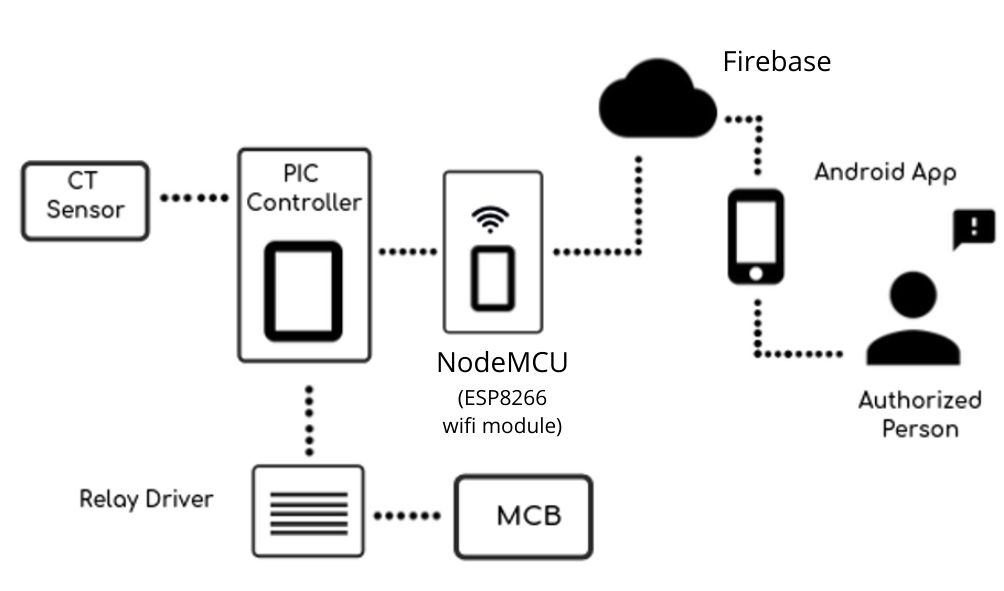
\includegraphics[width=\linewidth]{FirebaseAr.png}\\
	\caption{Basic Overview Diagram of Smart energy monitoring and controlling device}
	\label{fig:1.5}
\end{figure}
\begin{center}
Figure \ref{fig:1.5} Show Basic Overview Diagram of Smart energy monitoring and controlling device.
\end{center}

% -----------------                    Chapter 2: Literature Survey            ------------------------------

\newpage
\pagebreak
\vspace*{\fill}% * is needed here
\noindent
\makebox[\textwidth]{\textbf{\huge Literature Overview}}
\vfill


\newpage
\section{Literature Overview}
\fancyfoot[R]{\thepage}

\hspace{0.5cm} \textbf{2.1} Survey checking from,\emph{ "Design and implementation of Bluetooth energy meter”, (2012)}
By P. Shum, Y. C. Tong,Y. H. Sng, P. H. Chong and H. W. Kuek.\\

In above project report they defined present day electricity power dimension is constantly changing electronically and mechanical meters particularly in India and China. A wi-fi virtual power meter could simply extra green and handy to the meter analyzing task. Bluetooth era is taken into consideration as conversation era in above machine. And similarly they enforce it. By the usage of this machine person acquire information of power on the Bluetooth community wirelessly. \\

\hspace{0.2cm} \textbf{2.2} Gobinath. S, Gunasundari. N and Gowthami. P Worked on \emph{“IOT Based Energy Meter”} PIC Microcontroller calculating price \& displayed in Liquid Crystil Display and serial communique has been used to interface with the digital.

\hspace{0.2cm} \textbf{2.3} It is from \emph{  “IoT based energy meter reading, theft detection and Disconnection the use of Power optimization \& PLC modem ”, (Vol. 4, Issue 7, July 2015).}\\

By “Darshan Iyer N student of PES College of Engineering, Mandya, Karnataka, India”
In above paper explains the machine include PIC Microcontroller.The provided Energy meter machine minimize or almost removes the human dependecy in Electricity Checking. It is likewise useful in time period of pay of power invoice due to vital server is there. The consumer can screen and managed power intake in gadgets from an internet interface via way of means of supplying IP deal with of devices. This machine additionally for Theft detection of power meter \& it's tampering and It is especially focussing of power usages consumes and ship robbery locate records via way of means of the use of PLC modem.\\

\hspace{0.2cm} \textbf{2.4} Birendra Kumar Sahani 1, Tejashree Ravi 2, Aqib Javed Tamboli 3, Ranjeet Pisal four
They posted IRJET on April four 2017.\\

In this paper the concept of clever electricity meter the usage of IoT and Arduino had been introduced.\\


% -----------------                    Chapter 3: Introduction to Project domain            ------------------------------

\newpage
\pagebreak
\vspace*{\fill}% * is needed here
\noindent
\makebox[\textwidth]{\textbf{\huge Introduction to Project }}
\vfill

\newpage
\section{Internet of Things}
\fancyfoot[R]{\thepage}

\hspace{0.5cm}The marketplace for Internet utility increase could be very excessive these days.The IoT is a huge era that
permits us to create more than a few advantages to net packages. So, IoT is a group in which
all connected gadgets are related to the internet over community gadgets, routers for exchange of
information.IoT permits artifacts to be remotely operated thru present community infrastructure.IoT
is a completely powerful and insightful approach that gets rid of each human attempt and convenient
get entry to to bodily gadgets.In addition, this method has an self reliant control function
wherein no human touch might be managed via way of means of any gadget.

\begin{figure}[H]
	\centering
	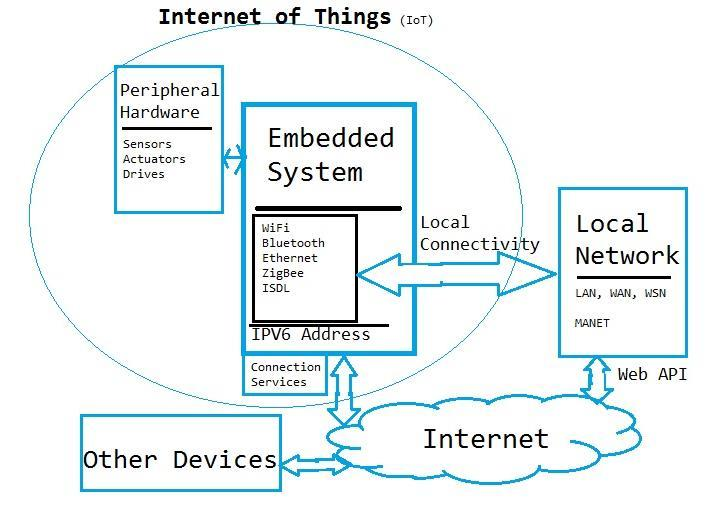
\includegraphics[width=\linewidth]{iot-structure.png}\\
	\caption{basic structure of Iot}
	\label{fig:3.1}
\end{figure}
\begin{center}
Figure \ref{fig:3.1} Show basic structure of Iot.
\end{center}

\hspace{0.5cm}The better than the discern demonstrates the houses of the special internet-primarily based totally equipment
and the sharing of statistics among them.Higher than the variety, consequently, is the property
of the planet throughout diverse modern-day technology.

\hspace{0.5cm}”Things” withinside the IoT context is a combination of software, hardware, information, and offerings.”Stuff”
might be addressed with an excellent fashion of gadgets which includes deoxyribonucleic acid evaluation equipment for environmental checking, electric clamps in coastal waters, Arduino chips in domestic development,
and lots of others.These gadgets collect beneficial statistics with the resource of plenty of present
technology and percentage this statistics among special gadgets.Examples encompass the HomeAutomation Program, which makes use of Wi-Fi or Bluetooth to percentage statistics among diverse domestic
gadgets.

\vspace{0.1in}
\textbf{\large{Features of IOT}}\\

\textbf{\large{Analysing:}} After connecting all of the applicable items, it takes a time period to evaluate
the statistics amassed and use it to make enterprise intelligence efficient.When we've got an
sincere view into the statistics amassed from those issues, then we opt to agree whether
our software functions an excellent gadget.\\

\textbf{\large{Connectivity:}} Connectivity refers back to the dedication of the suitable relation among all IoT and IoT community gadgets that need to be server or cloud. When connecting IoT
gadgets, excessive-pace digital conversation among gadgets and the cloud is needed to allow efficient, stable and both direction conversation.\\

\textbf{\large{Integrating:}}To raise the person revel in in addition to the IoT integrated into the special models.\\

\textbf{\large{Sensing:}} Detector gadgets utilized in IoT era notification and stay any extrade within
the context of the gadget and document on their status.IoT era transforms passive networks
into energetic networks.\\

\textbf{\large{Connectivity:}} Connectivity refers back to the dedication of the suitable relation among all IoT and IoT community gadgets that need to be server or cloud.When connecting IoT
gadgets, excessive-pace digital conversation among gadgets and the cloud is needed to allow efficient, stable and bi-directional conversation.\\

\textbf{\large{Active Engagement:}} The related era is created via way of means of IOT, or offerings for
energetic conversation with every different.\\

\subsection{Use of programming languages \& cloud IOT}
\subsubsection{Usage of programming languages in IOT}
\hspace{0.5cm} The IoT is these days one of the maximum well-known fields in era.Innovations in
this location are too smooth to maintain up, due to the fact increasingly more gadgets are being related to the
Internet each unmarried hour.We realize that those machines speak and switch information to and
from different computer systems over the Internet, however how do they perform internally?How and in what
language are those equipment configured to paintings simply as they need to be?IoT apps need to now no longer use any
difficult to understand languages that we've got by no means heard of.Usually, they use not unusualplace languages to function,
considering the fact that they normally use micro-computer systems which includes Raspberry PI.

\vspace{0.1in}
\textbf{\large{C language}}\\

\hspace{0.5cm}One of the maximum critical programming languages withinside the IoT gadget is the C.This may be
a certainly reasonably-priced layer of pc code on the lowest of the hardware.C has been the inspiration
of plenty of special languages writing commitments over the year.This makes the information
critical for all people in the IoT to return back.The reasoning at the back of this will be that there may be no
want for masses of method control.C is offered for nearly any superior embedded device
platform.C is procedural in preference to item-orientated because it has no essential capabilities.

\vspace{0.1in}
\textbf{\large{Java language}}\\

\hspace{0.5cm}Java is a programming language and it is very famous withinside the programming network. It’s the equal function that creates Java a top notch programming language for IoT projects.Com country that Java is the maximum famous language of IoT builders.Once a Java software is written, it is able to be run on any gadget that helps JVM, which includes smartphones, computers or even very small gadgets.The introduction
of the JME or the micro version has boosted the variety of builders.The important cognizance of
Java IoT builders as of these days is the Java SE Embedded, which could be very near the standard
version.

\vspace{0.1in}
\textbf{\large{Features of JAVA}}\\

\textbf{\large{Object Oriented }} ava may be effortlessly prolonged due to the fact it's far primarily based totally on an item model.Almost
the entirety in Java is an item.\\

\textbf{\large{Simple }} ava is supposed to be smooth to discover out.If you’re aware about the crucial concept of OOP
Java, it is probably smooth to master.\\

\textbf{\large{Portable }} Being architecture-impartial and having no implementation-established aspects
of the specification makes Java moveable.\\

\textbf{\large{Architecture-neutral }} Java compiler creates an architecture-impartial item file
format in which it creates the compiled code achievable on more than one processors, with the presence of a
Java runtime gadget.\\

\textbf{\large{Platform Independent }} Unlike numerous special programming languages in addition to C
and C++, as soon as Java is compiled, it isn't always compiled right into a platform-particular system, however rather
right into a platform-impartial pc reminiscence unit code.This pc reminiscence unit code is
allotted on line and brought from the Java Virtual Machine (JVM) on any platform on which it's far
running.\\

\textbf{\large{Secure }} Java is stable function permits the improvement of virus-loose, tamper-loose systems.Authentication strategies Quadratic degree supported public-key mystery writing.\\

\textbf{\large{Robust  }} Java makes a tribulation to do away with mistakess via way of means of accentuating on assemble time mistakess exams
and runtime exams withinside the important.\\

\textbf{\large{Javascript }} In 90s JavaScript evolved as a site-forming synthetic language. BrendanEich advanced JavaScript as syntax look like C, so no person imagined that JavaScript might play a
extreme position withinside the improvement of monetary software. JavaScript turned into created via way of means of ECMA International in 1997.\\

\begin{figure}[H]
	\centering
	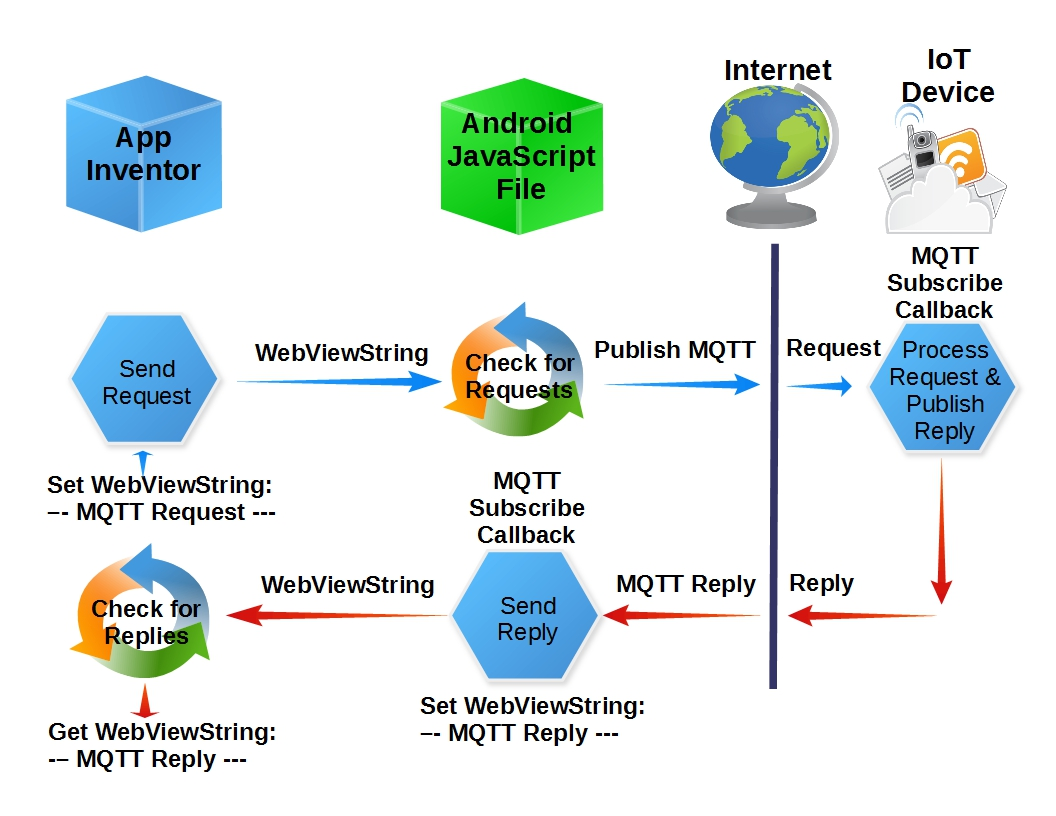
\includegraphics[width=\linewidth]{blockdiagram-1.jpg}\\
	\caption{Javascipt for Iot and android application}
	\label{fig:3.2.1}
\end{figure}
\begin{center}
Figure \ref{fig:3.2.1} Show Javascipt for android application.
\end{center}

\begin{itemize}
	\item Creation of the Standard Object Notations of JavaScript (JSON).
	\item Introduction of Node.Js in 2009 via way of means of Ryan Dahl. Node.Js performed a critical position in building
JavaScript internet servers the use of Google’s super-rapid JavaScript V8 engine. JavaScript is now
extensively utilized in cellular apps, internet pages and IoT systems.
\end{itemize}

\subsubsection{Cloud Platform}
\hspace{0.5cm} The Internet of Things is starting to remodel the day by day obligations of rectangular degree completed. The
community of gadgets (IoT) includes normal gadgets – bodily gadgets, vehicles, etc.
With integrated bodily science, software, sensors, and community assets, letting them collect,
ship and obtain information.The IoT generates an substantial quantity of big information, and
this successively locations an substantial pressure at the internet infrastructure. As a result, this forcescorporations to searching for answers to reduce strain and clear up their disadvantage to transferring
big quantities of information.\\

Cloud computing has brought the concept of information era, presenting quantifiability withinside the
shipping of organization packages and as a Service (SaaS) package. Corp. rectangular measures are
presently transfering their information working to the cloud. Some cloud companies will go away your
information to be transferred both thru your historical community affiliation or thru a fervent
direct hyperlink.The benefit of a direct hyperlink to the cloud can ensure that your information is
undisputed that the site visitors does now no longer pass the internet and consequently the exceptional of provider is often
managed.\\

\begin{figure}[H]
	\centering
	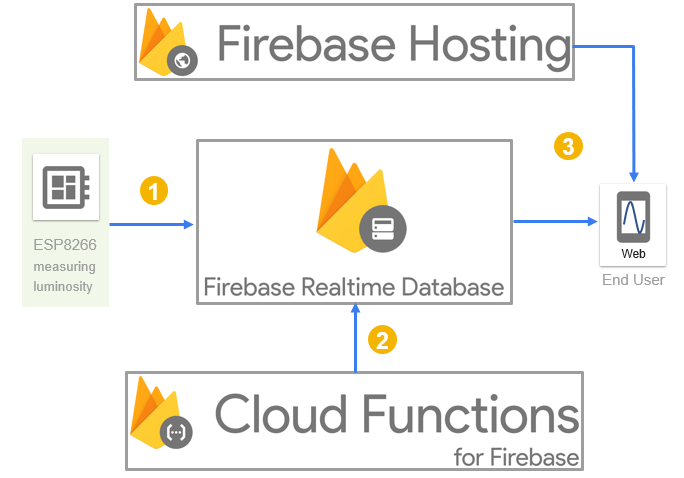
\includegraphics[width=\linewidth]{cloudsystem.png}\\
	\caption{Simple Cloud platform}
	\label{fig:3.2.2}
\end{figure}
\begin{center}
Figure \ref{fig:3.2.2} Show Simple Cloud platform.
\end{center}

\subsection{JAVA Language, C and CPP }
\hspace{0.5cm} Most IoT initiatives require the usage of a microcontroller or a pc tool. You want to
software this tool / microcontroller to attain the goal / output of your venture through operating
sure tasks. Then nearly all microcontrollers or different pc gadgets to be had at the market
assist C-language programming both solely or with assist for different languages such as
python. Another choice to software the tool is to apply meeting language, however it’s going to be a totally time-eating task.In a way. That shows, in case you realize C programming, so you could software nearly any
microcontroller efficiently.

In latest times, the IOT has grow to be omnipresent and is presently a desired
area in the developer network. According to Statista’s analysis, 1/2 of a dozen.21 million
IoT builders and five.36 million IoT builders are predicted to feature IoT withinside the subsequent 1/2 of-dozen
months.If you need to induce IoT to begin and are curious that the synthetic language will begin,
right here can be a listing of 11 not unusualplace programming languages used in IoT. C is the programming language that
become initially evolved for the programming of smartphone switches, can be a dependable and cheap
opportunity for the improvement of embedded structures. It’s fantastic due to its proximity
to device language.\\

It is a language of method and the program is checked and now no longer taken. The program written
in C could be very dependable and ascending, and processor independence creates it a robust rival to IoT
improvement. As a end result of C now no longer being a contract platform, it permits IoT builders to
reprocess code that may run on maximum structures.With the assist of suggestions, gaining access to and modifying
addresses in C is straightforward.

C++ is designed with a bias in the direction of device programming, embedded programming, resourcerestricted gadgets, and massive structures.

C++ can be a not unusualplace opportunity to the name of the game writing of embedded builders for Linux
structures.

Java is an related object-orientated language, and there are just a few hardware dependencies withinside the compiler that make it unmovable.Security is the primary problem in IoT; with GCF 8, Java’s Access Purpose API affords the brand new safety requirements and additionally the very best degree of networked coding and authentication that guarantees privacy.
All the Java object references are implicit suggestions that cannot be changed through the software program. This routinely excludes the capacity chance of operational infringements which may
necessarily reason the related software to save you all of as soon. In addition, connectivity
on the relevant degree of the IoT device is truly treated in Java with a complete set of
Apes genes, every of that's commonplace and freely to be had via open deliver.


\subsection{Working of IoT}
\hspace{0.5cm} The IoT device includes web-connected touchy gadgets that use embedded processors, sensors and communique hardware to gather, ship and act at the statistics they use from
their environments.IoT gadgets percentage the sensing detail statistics they acquire through connecting
to an related IoT entryway or a exclusive facet tool anyplace statistics is both despatched to
the cloud to be checked regionally. so those gadgets speak with a
form of related gadgets and act at the statistics they get from every different. Devices do maximum of
the paintings even as now no longer human intervention, despite the fact that humans circulate with gadgets — for example, line
them up, offer guidelines to them, or get entry to statistics.

Networking and communique protocols used with those web-enabled gadgets
depend, for the maximum part, at the specific IoT programs deployed.

\vspace{0.1in}
\subsection{Advantages of IoT}
\hspace{0.5cm}The IoT gives lots of advantages to organizations, sanctioning them:
\begin{itemize}
	\item tracking their enterprise workings
	\item enhancing purchaser engagement
	\item saving money and also time
	\item  enhancing employee quality of work
	\item combining and adapting enterprise devices and system 
	\item making better enterprise decisions and
	\item producing loads of revenue.
\end{itemize}

\begin{figure}[H]
	\centering
	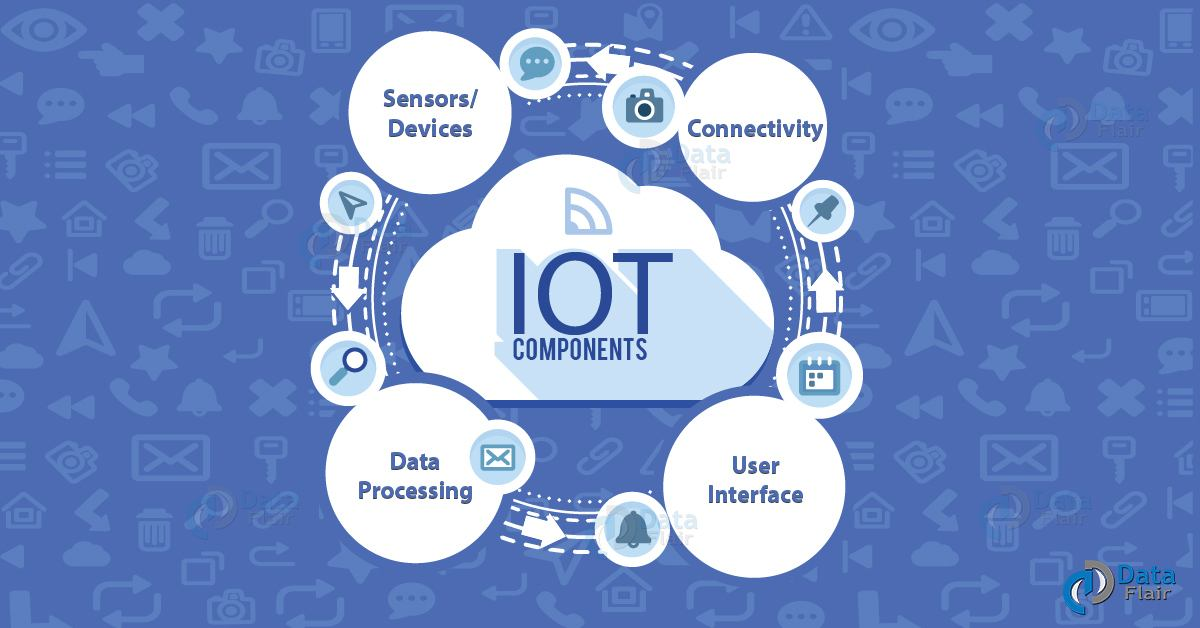
\includegraphics[width=\linewidth]{IOT-Components.jpg}\\
	\caption{IoT Basic sections}
	\label{fig:3.4}
\end{figure}
\begin{center}
Figure \ref{fig:3.4} Show Basic sections.
\end{center}

\subsection{Arduino IDE infromation}
\vspace{0.1in}
\begin{itemize}
	\item Arduino IDE is an companion diploma open-supply software program bundle this is often used
for writing and assembling code into the Arduino module.
	\item It is a politician Arduino software program bundle, developing code analyzing too easy so
that even an ordinary individual and not using a preceding technical statistics gets their toes moist with the
academic approach.
	\item A Range of Arduino modules on hand in addition to Arduino Uno, Mega, carver, Arduino small and masses of additional.
	\item Every of this carries a microcontroller at the board that is definitely coded and accepts
the statistics in the form of program.
	\item In this we can create program then we can compile it and then thecode will be added in arduino board.
	\item This placing helps every C and C++ languages.
\end{itemize}
The IDE surrounding overview of Arduino IDE


\begin{figure}[H]
	\centering
	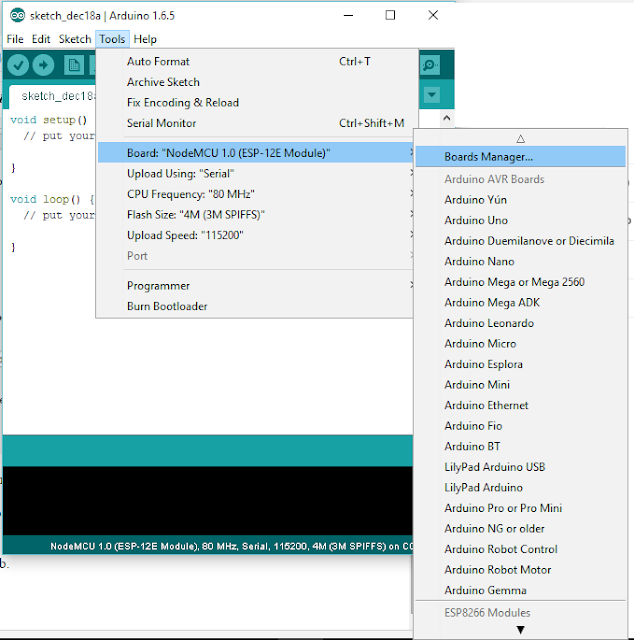
\includegraphics[width=14cm, height=11cm]{arduino-editor.png}\\
	\caption{Arduino IDE Editior Image }
	\label{fig:3.5}
\end{figure}
\begin{center}
Figure \ref{fig:3.5} Show Arduino IDE Editior Overview.
\end{center}

\subsubsection{Benefits of Arduino IDE}

\vspace{0.1in}
\textbf{\large{Multi-Platform Application}}\\

\hspace{0.5cm} Arduino IDE works on 3 desired working structures: Windows OS, Linux and Mac OS .
In these whatever packages we want we can add it into this on any os.

\vspace{0.1in}
\textbf{\large{Board Management}}\\

\hspace{0.5cm} Arduino IDE contains a board control module with anyplace customers select the board, microprocessor
they want to paintings with instantly. If they need to alternate it, they’re simply going to do it from the
drop-down menu. Modifying their desire collectively routinely updates the PORT data with
the statistics they've at the relevance of the brand new board.

\vspace{0.1in}
\textbf{\large{Straight forward Sketching }}\\

\hspace{0.5cm}With Arduino IDE, customers will produce packages called sketches of a textual content editordesigned place unit. The approach can be an smooth one, despite the fact that it’s loads of bells and whistles
that create loads of interactive expertise.

\vspace{0.1in}
\textbf{\large{Vast Library }}\\

\hspace{0.5cm}Arduino IDE has over seven-hundred integrated libraries. These had been written and shared through
contributors of the Arduino network who can be utilized by exclusive customers for his or her very own purposes
even as now no longer having to installed. This permits coders to have a unique size to
their programs. While Arduino IDE is supposed especially for Arduino , it at the same time helps thirdparty hardware connections. This makes the usage of the equipment lots greater in-intensity than
restrained to proprietary boards.


% -----------------                    Chapter 4: Project Design Flow            ------------------------------

\newpage
\pagebreak
\vspace*{\fill}% * is needed here
\noindent
\makebox[\textwidth]{\textbf{\huge Project Design Flow}}
\vfill


\newpage
\section{Overview of project}
\fancyfoot[R]{\thepage}

\hspace{0.5cm}The IOT idea permits consumer to attach the traditional everyday gadgets with each other to the web internet. The gadgets linked thru concept of iot are regularly analyzed from anywhere. The iot concept presents the essential infrastructure and possibilities to create a connection among the bodily international and computers - primarily based totally systems. The concept has been getting significance with plenty of and plenty of wi-fi gadgets which can be increasing in a timely fashion in the market. The hardware gadgets are linked with each other anywhere in the internet. The E.S.P. 8266 Wi-Fi module applied withinside the gadget presents the connections with the internet within the gadget.\\

This mission describes the upgradation of load power utilization readings on the internet. The deliberate gadget layout removes the involvement of human in power maintenance. The consumer will display power intake in watts from a web site via way of means of supplying a channel identityentification for the burden. It can be used in anywhere for development, security, making life more easy. Wi-Fi unit plays IOT operation via way of means of inflicting power facts of the burden to the web site which may be accessed thru the channel identityentification of the device. in the projected gadget, consumer will do electricity control via way of means of understanding power utilization time to time. This projected gadget makes use of an Arduino controller. The unit this is generated might be displayed at the web site thru the Wi-Fi module.\\

\subsection{Project Architecture}
\hspace{0.5cm}Project design mainly consists of Hardware units namely (controller, sensor, relay, wifi module), cloud and mobile application. Hardware setup used to collect sensor data and send it to the cloud and after that mobile application downloads that data and displays it in a standard format And is able to send signal from the app to the network over the Internet.\\


\begin{figure}[H]
	\centering
	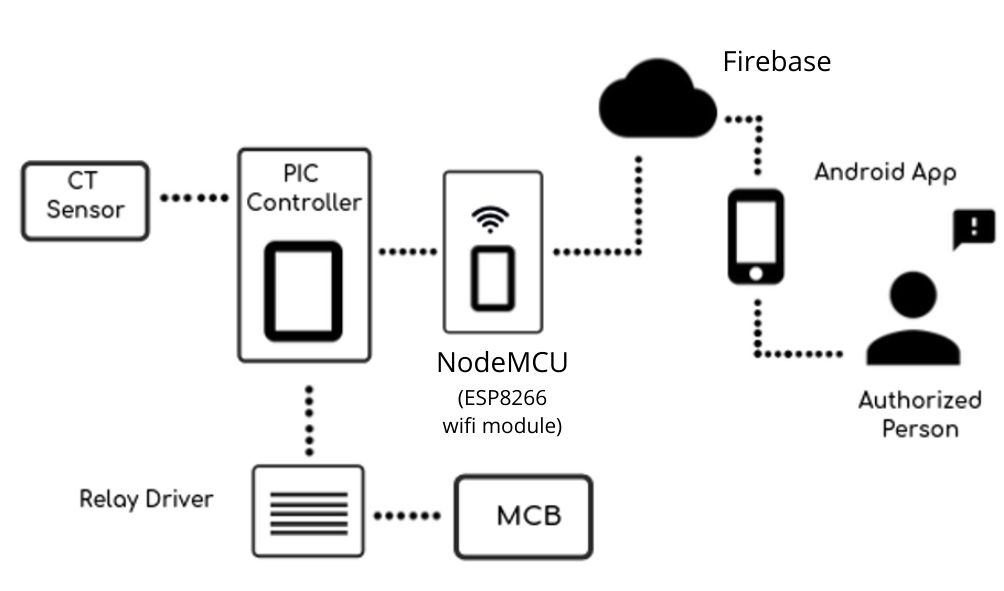
\includegraphics[width=\linewidth]{FirebaseAr.png}\\
	\caption{System Overview}
	\label{fig:4.1}
\end{figure}
\begin{center}
Figure \ref{fig:4.1} Show Overview of System.
\end{center}

\subsection{Building blocks of Project}
\hspace{0.5cm}This strategic specific incorporates 3 developing square 1.hardware 2.Cloud 3. Portable utility.We interface sensor, transfer and LCD with the controller. ESP module through method of methods for the utilization of sequential Communication Send measurements to the cover over a net. What's more, bring insights in android utility the use of an unmistakable library.\\

\subsubsection{Project Functional Description }
\hspace{0.5cm}This crucial split into 3 components explicitly equipment arrangement, cloud and cell utility. Equipment arrangement specifically incorporates controller, WiFi module, sensor circuit, hand-off circuit and LCD. Controller well interfaced with all unique factor of circuit. We have utilized current transformer for detecting current. Hand-off circuit with ULN 2003 transfer main impetus IC for controlling computerized on/off contraptions. Correspondence among Wifi module and controller is built up through sequential correspondence. Code is written in NodeMCU controller for power computation and moving the insights to cloud.\\

Firebase is open flexibly cloud transporter in which we have made channel. It creates channel ID with look at and compose API keys. Two fields withinside the channel are utilized for power and On/off controlling of gadget. 

Android studio is utilized for utility turn of events. In that Volley, Lecho and Firebase libraries are utilized. Card see is utilized to set up 4 basic games explicitly on/off, Readings and About. Information is brought in android utility with the help of compose and examin keys.

\subsection{Project (Hardware/Software) Specifications}
\hspace{0.5cm} Hardware development of system consist of hardware components selection and interfacing them together and develop real time system. For that purpose di-erent data sheets are referred. Hardware development include real time data acquisition of proposed system.\\

\subsubsection{NodeMCU H/W}

\begin{figure}[H]
	\centering
	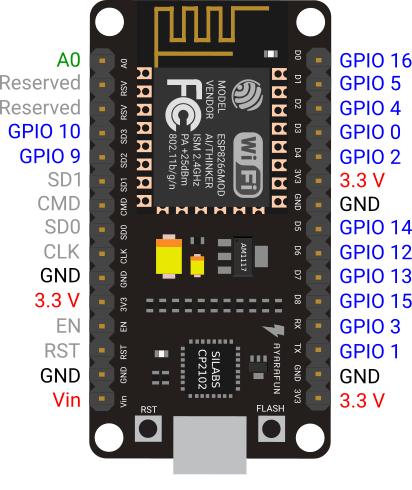
\includegraphics[width=5cm, height=6cm]{NodeMCU.png}\\
	\caption{NodeMCU}
	\label{fig:4.3.1}
\end{figure}
\begin{center}
Figure \ref{fig:4.3.1} NodeMCU.
\end{center}


\hspace{0.5cm} NodeMCU is an open-gracefully firmware and improvement bundle that encourages you to model or develop IoT devices. This comprises of the firmware that runs at the Espressif Systems ESP8266 Wi-Fi SoC and the equipment this is principally founded absolutely on theESP-12 board. The product program utilizes the language of the Lua content. \\

\hspace{0.5cm} There's also 128 KB of RAM and four MB of Flash memory (for application and records stockpiling) essentially adequate to address the huge strings that make up the web pages, the JSON/XML documents, and the entire parcel we're setting on IoT devices today. \\

\hspace{0.5cm} The ESP8266 incorporates 802.11b/g/n HT40 Wi-Fi handset all together that it can't handiest interface with a WiFi people group and talk with the Internet, anyway additionally can establishment its very own network, allowing various devices to append quickly to it. \\

\hspace{0.5cm} Force is given to the ESP8266 NodeMCU through an on-board MicroB USB connector.\\

\hspace{0.5cm} The ESP8266 NodeMCU has a total of 17 GPIO pins harmed out to the pin headers on every aspects of the improvement board. Such pins can be assigned to all method of fringe errands, including: \\
ADC channel – A 10-bit ADC channel.\\
UART interface \\
PWM outputs \\
SPI, I2C and I2S interface – SPI and I2C interface to connect a wide range of sensors and peripherals. \\

I2S interface – I2S interface on the off chance that you need to add sound to your venture.\\

\hspace{0.5cm}The NodeMCU has buttons.The different FLASH button withinside the backside left nook is the down load button used to improve the firmware.\\

\subsubsection{Current Transformer}

\begin{figure}[H]
	\centering
	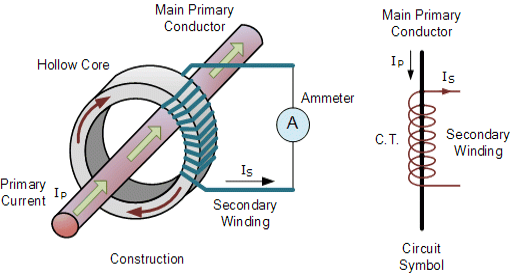
\includegraphics[width=8cm, height=6cm]{ctsensor.png}\\
	\caption{CT Sensor}
	\label{fig:4.3.3}
\end{figure}
\begin{center}
Figure \ref{fig:4.3.3} Current Transformer sensor.
\end{center}

\hspace{0.5cm}The Current Transformer CT is a sort of "gadget transformer" that is built up 
to give a rotating current in its auxiliary winding that is corresponding to the advanced 
being estimated in its main windings. Current transformers diminish the unnecessary voltage flows 
to a far lessening cost and offer a green way of ably following the genuine electric present day streaming in an AC transmission line the utilization of a mainstream current meter. The first of working 
of an essential present day transformer is common particular from that of an ordinary voltage transformer.\\ 

Current transformers can "step-down" present day stages from many amperes right down to a 
well known yield of a perceived proportion to both five Amps or 1 Amp for common activity. Along these lines, little 
also, right gadgets and control contraptions might be utilized with CT's because of this they are 
protected farfar from any over the top voltage vitality follows. There are some of metering applications 
what's more, utilizes for present day transformers like with Wattmeter's, vitality thing meters, watt-hour meters, 
securing transfers, venture loops in attractive circuit breakers and MCB's.\\

\textbf{\large{key notes of Current transformer}}\\ 
\begin{itemize}
	\item Test voltage For Ring (Window) kind  CT is 4KV 50 Hz for 1 min (besides  for 50/30 CTtype and 50/50 CT type  in which check voltage is 3KV 50 Hz for 1 min) For Wound kind  CT is 3KV 50 Hz for 1 min.
	\item Operating frequency is 50Hz / 60 Hz.
	\item Rated number one score is 1Ato 7500A.
	\item Rated secondary output is 5Astandard (1Aon request)
	\item Rated burden is 1, 1.25, 1.five, 2.five, three.75, five, 7.five, 10, 12.five, 15, 20, 30, 45, 60, a hundred VA

\end{itemize}

\subsubsection{LCD 16x2}
\hspace{0.5cm}Fluid Crystal Display show is an advanced show module and find some of uses. A 16x2 LCD shows are essential module and are regularly used in different 
contraptions and computerized circuits. These modules are chosen more than seven portions and diverse avialable multi stage LEDs. The intentions are LCDs are efficient, without trouble programmable, have no 
issue of demonstrating remarkable or even custom characters rather than in seven portions, movements 
what's more, a lot of more prominent. A 16x2 LCD way it's miles used to show sixteen characters with regards to line and there are 
2 such follows to be had. In this LCD each individual is shown in 5x7 frameworks of pixels. This 
LCD has registers which can be Command and Data.\\

\textbf{\large{Key points of LCD}}\\ 
\begin{itemize}
	\item Operating Voltage  4.7V to five.3V
	\item Current intake 1mA with out backlight.
	\item Alphanumeric LCD show module, manner can show alphabets and numbers.
	\item Consists of such rows and every row can print sixteen characters
	\item Each person is constructed via way of means of a five x eight field pixel
	\item It can paintings eight-bit and 4-bit mode
\end{itemize}

\subsubsection{Relay Module}
\hspace{0.5cm} Transfer is a switch, that opens and shuts the circuit electrically. It utilizes truth of electromagnetism from little voltage to offer better voltages. It has 2 essential contacts i.E. NO Normally Open and NC Normally Closed. When enter voltage is executed all through transfers loops, Normally Closed changes in accordance with Normally Open and Normally Open acclimations to Normally Closed. When enter voltage is actualized, the hand-off is invigorated. Hand-off has various capacities e.G. it can be utilized for exchanging better voltage devices to littler voltage devices. In any case, it have to now never again be used in vitality ingesting contraptions. It has a gigantic assortment of utilizations. It might be applied in household machines, advanced circuits in which there's an interest of security, mechanical autonomy for controlling its engines from the correct development and diverse more prominent.\\


\textbf{\large{Key points of relay module}}\\ 
\begin{itemize}

\item Contact current 10A and 250V AC or 30V DC. 
\item Each channel has sign LED. 
\item Loop voltage 12V with regards to channel. 
\item Unit running voltage five-12 V 
\item Information sign three-five V for each channel. 
\item Three pins for ordinarily open and shut for each channel.
	
\end{itemize}

\subsubsection{Pic Microcontroller}
\hspace{0.5cm} PIC (normally said as "pick") is an own hover of family members of microcontrollers made through method of methods for Microchip Technology, got from the PIC1650 from the outset advanced by means of method of methods of GIMD. The call PIC as a matter of first importance refered to Peripheral Interface Controller, and is as of now 
expanded as Programmable Intelligent Computer. The principal parts of the own hover of family members have been to be had 
in 1976; by means of method of methods for 2013 the association had dispatched more prominent than twelve billion man segments, used in a 
broad kind of installed frameworks.\\

\subsubsection{ PICKIT }

\begin{figure}[H]
	\centering
	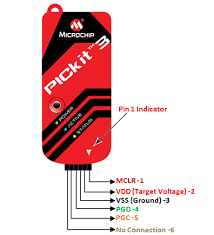
\includegraphics[width=5cm, height=6cm]{pickit.png}\\
	\caption{ Image of pickit }
	\label{fig:4.3.6}
\end{figure}
\begin{center}
Figure \ref{fig:4.3.6} pickit 3.
\end{center}

\hspace{0.5cm} The PICkit three developer/debugger (see Figure 1-1) is a straightforward, low-cost in-circuit debugger this is overseen through method of methods for a PC running MPLAB IDE (v8.20 or more noteworthy) programming program on a Windows R stage. The PICkit three developer/debugger is a fundamental a piece of the improvement architect's toolsuite. The product usage can extend from programming program improvement to equipment combination.\\ 

The PICkit three developer/debugger is a debugger gadget utilized for equipment and programming program improvement of Microchip PIC R microcontrollers (MCUs) and dsPIC R Digital Signal Controllers (DSCs) which can be fundamentally founded absolutely on In-Circuit Serial ProgrammingTM (ICSPTM) and Enhanced In-Circuit Serial Programming 2-rope sequential interfaces. Notwithstanding debugger works, the PICkit three software engineer/debugger gadget moreover can be utilized as an improvement developer. \\

The debugger gadget executes code like a genuine instrument as it utilizes an apparatus with builtin copying hardware, instead of a one of a kind debugger chip, for imitating. All to be had elements of a given instrument are close by intelligently, and might be set and changed by means of method of methods for the MPLAB IDE interface.\\

\subsection{Software Specification}

\subsubsection{ Arduino programming}
\hspace{0.5cm} Arduino applications are composed withinside the Arduino Integrated Development Environment (IDE). 
Arduino IDE is an extraordinary programming program running to your machine that allows in you to carefully record outlines 
(equivalent word for programming in Arduino language) for elite Arduino sheets. The Arduino programming language is principally founded absolutely on a totally simple equipment programming language known as handling, 
that is a lot of like the C language. After the funny cartoon is composed withinside the Arduino IDE, it should be 
transferred at the Arduino board for execution. \\

The initial phase in programming the Arduino board is downloading and placing in the Arduino 
IDE. The open flexibly Arduino IDE runs on Windows OS, Mac OS X, and Linux.\\

The NodeMCU is a improvement board offering the famous ESP8266 WiFi chip. As it
turns out, you could software the ESP8266 much like another microcontroller. Its apparent gain over the Arduino or PIC is that it is able to with ease hook up with the Internet through WiFi. However,
the ESP8266 breakout board has restricted pins despite the fact that the chip itself has a whole lot of output ports.
The NodeMCU solves this trouble via way of means of offering 10 GPIO pins every able to the use of PWM, I2C
and 1-cord interface.\\

\subsubsection{ Specifications of Android studio }
\hspace{0.5cm} Android Studio is the widely recognized IDE for Android
software improvement, primarily based totally on IntelliJ IDEA of improvement . On pinnacle of IntelliJ’s powerful
code editor and developer gear, Android Studio offers even greater capabilities that boom your
productiveness while constructing Android apps.\\

\textbf{\large{ Key points of Android Studio}}\\ 
\begin{itemize}
	\item A bendy Gradle-primarily based totally constructing machine.
	\item A speedy in addition to feature-wealthy emulator.
	\item A unified surroundings in which consumer can increase for all Android devices.
	\item Instant Run to push modifications to customers jogging app with out constructing a brand new APK.
	\item Code templates in addition to GitHub integration that will help you construct not unusualplace app capabilities and
import pattern coding.
	\item Extensive trying out gear or frameworks.
\end{itemize}

\subsubsection{MPLAB Software}
\hspace{0.5cm} The PIC microcontroller programming is accomplished through ‘MP-Lab’ software program. It is used for pic microcontroller to simulate the working circuit of pic controller. In this software we can write code for pic controller and simulate the  function of controller. we can also debug the code of program of pic and we can push the code of pic into pic by using this software and connector.\\

We use MP-Lab software for programming PIC-Microcontroller. MP-Lab is integrated development environment and microchip is integrated within MP-Lab. Microchip Software and hardware tools embedded in microchip.
Components of MPLab IDE\\
Since MPLab has variety of software and hardware tools for system configuration MPLAB has buit-in components and plug-in models.\\
Project Manager:
 It is a  communicator between the IDE and language tools. It provides integration.\\

Editor: 
It is a text editor used by programmers that serves as a window into the debugger.\\
Linker: 
for linking single file we can use assembler or it can be used with linker to build project from seprate source files. Linker set the compiled code into memory area.\\
Debugger-
 The Microchip debugger permits breakpoints, single venturing, watch windows and all the highlights of a cutting edge debugger for the MPLAB IDE. It works related to the manager to reference data from the objective being fixed back to the source code.
Execution Engines: 
They are software simulators.\\

\subsubsection{Proteus Software}
\hspace{0.5cm}The Proteus Design Suite software program is a proprietary software program device suite used broadly speaking for digital layout and automation. The software program is used in particular via way of means of the digital designers engineers
in addition to technicians for growing schematics and digital prints to fabricate published circuitboards PCB’s.\\

The PCB Layout module is routinely given connectivity facts withinside the shape of a
netlist from the schematic seize module. It applies this facts, collectively with the consumer
distinctive layout regulations and diverse layout automation gear, to help with blunders unfastened board layout.
PCB’s of as much as sixteen copper layers may be produced with layout length restricted via way of means of product configuration.\\


\subsubsection{Code1: Android Application}
\textbf{\large{Login . java}}\\ 

\begin{lstlisting}[frame=single]
package com.example.power_control;

import androidx.appcompat.app.AppCompatActivity;

import android.content.Intent;
import android.os.Bundle;
import android.text.TextUtils;
import android.os.Handler;
import android.view.View;
import android.widget.Button;
import android.widget.EditText;
import android.widget.ProgressBar;
import android.widget.TextView;
import android.widget.Toast;
import android.widget.RelativeLayout;

import androidx.annotation.NonNull;
import com.google.android.gms.tasks.OnCompleteListener;
import com.google.android.gms.tasks.Task;
import com.google.firebase.auth.AuthResult;
import com.google.firebase.auth.FirebaseAuth;

public class Login extends AppCompatActivity {

    EditText mEmail,mPassword;
    Button mLoginBtn;
    TextView mCreateBtn;
    ProgressBar progressBar;
    FirebaseAuth fAuth;

    RelativeLayout rellay1, rellay2;
    Handler handler =new Handler();
    Runnable runnable = new Runnable() {
        @Override
        public void run() {
            rellay1.setVisibility(View.VISIBLE);
            rellay2.setVisibility(View.VISIBLE);
        }
    };

    public class Login {
        public String username,email,phoneno;

        public Login(){

        }
    }

    public Login(String username, String email, String phoneno) {
        this.username = username;
        email = email;
        phoneno = phoneno;
    }


    @Override
    protected void onCreate(Bundle savedInstanceState) {
        super.onCreate(savedInstanceState);
        setContentView(R.layout.activity_login);

        mEmail = findViewById(R.id.et_email1);
        mPassword = findViewById(R.id.et_pass1);
        progressBar = findViewById(R.id.progressBar);
        fAuth = FirebaseAuth.getInstance();
        mLoginBtn = findViewById(R.id.btn_login);
        mCreateBtn = findViewById(R.id.btn_signupnow);

        rellay1 = findViewById(R.id.rellay1);
        rellay2 = findViewById(R.id.rellay2);

        handler.postDelayed(runnable, 2000);

        mLoginBtn.setOnClickListener(new View.OnClickListener() {
            @Override
            public void onClick(View v) {

                String email = mEmail.getText().toString().trim();
                String password = mPassword.getText().toString().trim();

                if (TextUtils.isEmpty(email)) {
                    mEmail.setError("Email is Required.");
                    return;
                }

                if (TextUtils.isEmpty(password)) {
                    mPassword.setError("Password is Required.");
                    return;
                }

                if (password.length() < 6) {
                    mPassword.setError("Password Must be >= 6 Characters");
                    return;
                }

                progressBar.setVisibility(View.VISIBLE);
                if (FirebaseAuth.getInstance().getCurrentUser() != null)
                {
                    finish();
                    startActivity(new Intent(Login.this, MainActivity.class));
                }
                else {
                    fAuth.signInWithEmailAndPassword(email,password).addOnCompleteListener(new OnCompleteListener<AuthResult>() {
                        @Override
                        public void onComplete(@NonNull Task<AuthResult> task) {
                            if(task.isSuccessful()){
                                Toast.makeText(Login.this, "Logged in Successfully", Toast.LENGTH_SHORT).show();
                                startActivity(new Intent(getApplicationContext(),MainActivity.class));
                            }else {
                                Toast.makeText(Login.this, "Error ! " + task.getException().getMessage(), Toast.LENGTH_SHORT).show();
                                progressBar.setVisibility(View.GONE);
                            }

                        }
                    });
                }

                // authenticate the user


            }
        });

        mCreateBtn.setOnClickListener(new View.OnClickListener() {
            @Override
            public void onClick(View v) {
                startActivity(new Intent(getApplicationContext(),Signup.class));
            }
        });


    }

}

\end{lstlisting}

\textbf{\large{Signup . java}}\\ 

\begin{lstlisting}[frame=single]

package com.example.power_control;

import androidx.appcompat.app.AppCompatActivity;

import android.os.Bundle;
import android.os.Handler;
import android.text.TextUtils;
import android.view.View;
import android.content.Intent;
import android.widget.Button;
import android.widget.EditText;
import android.widget.ProgressBar;
import android.widget.TextView;
import android.widget.Toast;
import android.widget.RelativeLayout;

import androidx.annotation.NonNull;

import com.google.android.gms.tasks.OnCompleteListener;
import com.google.android.gms.tasks.Task;
import com.google.firebase.auth.AuthResult;
import com.google.firebase.auth.FirebaseAuth;
import com.google.firebase.database.DatabaseReference;
import com.google.firebase.database.FirebaseDatabase;

public class Signup extends AppCompatActivity {

    EditText mUsername,mEmail,mPassword,mPhone;
    Button mRegisterBtn;
    TextView mLoginBtn;
    FirebaseAuth fAuth;
    ProgressBar progressBar;
    DatabaseReference databaseReference;
    FirebaseDatabase firebaseDatabase;


    RelativeLayout rellay3;
    Handler handler =new Handler();
    Runnable runnable = new Runnable() {
        @Override
        public void run() {
            rellay3.setVisibility(View.VISIBLE);
//            rellay2.setVisibility(View.VISIBLE);
        }
    };

    @Override
    protected void onCreate(Bundle savedInstanceState) {
        super.onCreate(savedInstanceState);
        setContentView(R.layout.activity_signup);

        mUsername   = findViewById(R.id.et_username);
        mEmail      = findViewById(R.id.et_email);
        mPassword   = findViewById(R.id.et_pass);
        mPhone      = findViewById(R.id.et_phone);
        mRegisterBtn= findViewById(R.id.btn_signin);
        mLoginBtn   = findViewById(R.id.tv_logins);


        databaseReference = FirebaseDatabase.getInstance().getReference("powercontrol");
        fAuth = FirebaseAuth.getInstance();


        rellay3 = findViewById(R.id.rellay3);
//        rellay2 = (RelativeLayout) findViewById(R.id.rellay2);

        handler.postDelayed(runnable, 1000);


        progressBar = findViewById(R.id.progressBar);

        if(fAuth.getCurrentUser() != null){
            startActivity(new Intent(getApplicationContext(),MainActivity.class));
            finish();
        }




        mRegisterBtn.setOnClickListener(new View.OnClickListener() {
            @Override
            public void onClick(View v) {

                final String email = mEmail.getText().toString().trim();
                String password = mPassword.getText().toString().trim();
                final String username = mUsername.getText().toString();
                final String phoneno = mPhone.getText().toString();

                if(TextUtils.isEmpty(email)){
                    mEmail.setError("Email is Required.");
                    return;
                }

                if(TextUtils.isEmpty(password)){
                    mPassword.setError("Password is Required.");
                    return;
                }

                if(password.length() < 6){
                    mPassword.setError("Password Must be >= 6 Characters");
                    return;
                }

                if(TextUtils.isEmpty(username)){
                    Toast.makeText(Signup.this,"Please enter username",Toast.LENGTH_SHORT);
                }
                if(TextUtils.isEmpty(phoneno)){
                    mPassword.setError("Phone Number is Required.");
                    return;
                }

                progressBar.setVisibility(View.VISIBLE);

                fAuth.createUserWithEmailAndPassword(email,password).addOnCompleteListener(new OnCompleteListener<AuthResult>() {
                    @Override
                    public void onComplete(@NonNull Task<AuthResult> task) {
                        if(task.isSuccessful()){

                            Login info = new Login(
                                    username,
                                    email,
                                    phoneno
                            );

                            FirebaseDatabase.getInstance().getReference("powercontrol")
                                    .child(FirebaseAuth.getInstance().getCurrentUser().getUid())
                                    .setValue(info).addOnCompleteListener(new OnCompleteListener<Void>() {
                                @Override
                                public void onComplete(@NonNull Task<Void> task) {

                                    Toast.makeText(Signup.this, "Registration Complete", Toast.LENGTH_SHORT).show();
                                    startActivity(new Intent(getApplicationContext(),MainActivity.class));
                                }
                            });



                            Toast.makeText(Signup.this, "User Created.", Toast.LENGTH_SHORT).show();
                            startActivity(new Intent(getApplicationContext(),MainActivity.class));

                        }else {
                            Toast.makeText(Signup.this, "Error ! " + task.getException().getMessage(), Toast.LENGTH_SHORT).show();
                            progressBar.setVisibility(View.GONE);

                        }
                    }
                });
            }
        });

        mLoginBtn.setOnClickListener(new View.OnClickListener() {
            @Override
            public void onClick(View v) {
                startActivity(new Intent(getApplicationContext(),Login.class));
            }
        });

    }
}


\end{lstlisting}


\textbf{\large{MainActivity . java}}\\ 

\begin{lstlisting}[frame=single]

package com.example.power_control;

import androidx.annotation.NonNull;
import androidx.appcompat.app.AppCompatActivity;

import android.content.Intent;
import android.graphics.Color;
import android.os.Bundle;
import android.view.View;
import android.widget.Button;
import android.widget.TextView;

import com.google.firebase.auth.FirebaseAuth;
import com.google.firebase.database.DataSnapshot;
import com.google.firebase.database.DatabaseError;
import com.google.firebase.database.DatabaseReference;
import com.google.firebase.database.FirebaseDatabase;
import com.google.firebase.database.ValueEventListener;

public class MainActivity extends AppCompatActivity {

    TextView temp,temp1,temp2;
    Float temperature;
    Button btn1,btn2,btn3,btn4;

    boolean check = false;
    DatabaseReference derf;
    String status;
    private int flag = 0;

    @Override
    protected void onCreate(Bundle savedInstanceState) {
        super.onCreate(savedInstanceState);
        setContentView(R.layout.activity_main);

        temp = findViewById(R.id.tv_val);
        temp1 = findViewById(R.id.tv_automanu);

        btn1 = findViewById(R.id.btn_node1);
        btn2 = findViewById(R.id.btn_node2);
        btn3 = findViewById(R.id.btn_node3);
        btn4 = findViewById(R.id.btn_node4);


        derf= FirebaseDatabase.getInstance().getReference();
        derf.addValueEventListener(new ValueEventListener() {
            @Override
            public void onDataChange(@NonNull DataSnapshot dataSnapshot)
            {
                status=dataSnapshot.child("power").getValue().toString();
//                temperature=Float.parseFloat(status);
//                temp.setText(status+" W");
//
                temp.setText(status+"  W");
//                temp.setText(status+" \u2109");
            }

            @Override
            public void onCancelled(@NonNull DatabaseError databaseError) {

            }
        });

        // Write a message to the database
        FirebaseDatabase database = FirebaseDatabase.getInstance();
        DatabaseReference myRef = database.getReference("message");

        myRef.setValue("Hello, World!");


    }


    public void logout(View view) {
        FirebaseAuth.getInstance().signOut();//logout
        startActivity(new Intent(getApplicationContext(),Login.class));
        finish();

    }

    public void autom(View view) {
        temp1.setText("Automatic");
        derf.child("Mode").setValue("Automatic");
    }

    public void manua(View view) {
        temp1.setText("Manual");
        derf.child("Mode").setValue("Manual");
    }

    public void nod1(View view) {

        if (flag == 0) {
            flag = 1; // 1 => Button ON
            btn1.setBackgroundColor(Color.RED);
            derf.child("Node1").setValue("OFF");

        } else {
            flag = 0; // 0 => Button OFF
            btn1.setBackgroundColor(Color.GREEN);
            derf.child("Node1").setValue("ON");
        }
    }

    public void nod2(View view) {

        if (flag == 0) {
            flag = 1; // 1 => Button ON
            btn2.setBackgroundColor(Color.RED);
            derf.child("Node2").setValue("OFF");
        } else {
            flag = 0; // 0 => Button OFF
            btn2.setBackgroundColor(Color.GREEN);
            derf.child("Node2").setValue("ON");
        }
    }

    public void nod3(View view) {

        if (flag == 0) {
            flag = 1; // 1 => Button ON
            btn3.setBackgroundColor(Color.RED);
            derf.child("Node3").setValue("OFF");
        } else {
            flag = 0; // 0 => Button OFF
            btn3.setBackgroundColor(Color.GREEN);
            derf.child("Node3").setValue("ON");
        }
    }

    public void nod4(View view) {

        if (flag == 0) {
            flag = 1; // 1 => Button ON
            btn4.setBackgroundColor(Color.RED);
            derf.child("Node4").setValue("OFF");
        } else {
            flag = 0; // 0 => Button OFF
            btn4.setBackgroundColor(Color.GREEN);
            derf.child("Node4").setValue("ON");


        }
    }
}

\end{lstlisting}


% -----------------                    Chapter  5. Project Implementation            ------------------------------

\newpage
\pagebreak
\vspace*{\fill}% * is needed here
\noindent
\makebox[\textwidth]{\textbf{\huge Project Implementations}}
\vfill


\newpage
\section{Project Implementation view}
\fancyfoot[R]{\thepage}

\subsection{Design methodology of the project}
\hspace{0.5cm}By using CT sensor we are going to measure current flowing through a wire from   which we can calculate the power consumption by using the formula: 
\begin{center}
                  Power = current(Rms) X voltage(Rms)
\end{center}
For that we  are need to calibrate CT sensor first , after calibration of sensor it can be interfaced  to the microcontroller.We need to convert analog data coming from  CT sensor to Digital using  ADC (Analog to Digital convertor) microcontroller.

Based upon threshold the microcontroller will priories each electric node and control them so that  power consumption will not exceeds. Collected records is displayed on LCD and despatched to the cloud for evaluation and observation. Later we fetch records in an android software and displayed it.

For monitoring and controlling system by using android app.We are connecting android app with cloud with use of authentication token and api key of cloud.To show Power Consumption.

\begin{figure}[H]
	\centering
	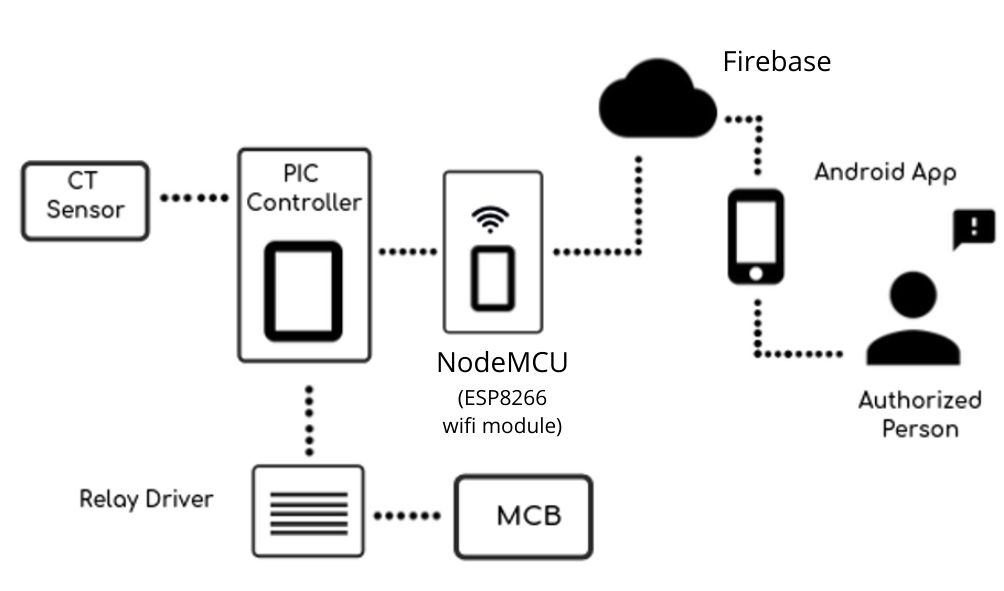
\includegraphics[width=\linewidth]{FirebaseAr.png}\\
	\caption{Design Methodology}
	\label{fig:5.1}
\end{figure}
\begin{center}
Figure \ref{fig:5.1} Show Design Methodology.
\end{center}

\subsubsection{Project requirement}
\hspace{0.5cm}The primary challenge necessities are a computer or laptop with eight GB of RAM and an OS hooked up. Android cell model five.0(Lollipop) and above. Android Studio model 3.6 for the improvement of applications. Arduino IDE model 1.eight.10 hooked up on laptop. MP lab x is hooked up for your laptop. StarUML software program for object-orientated design. USB cable A male to B male to unload the code into the \% controller. Diptrace software program to be hooked up for pcb design.\\

\subsubsection{System Architecture of Project}
\hspace{0.5cm} System architecture’s blocks are proven in discern underneath and interconnection among them.\\

\begin{figure}[H]
	\centering
	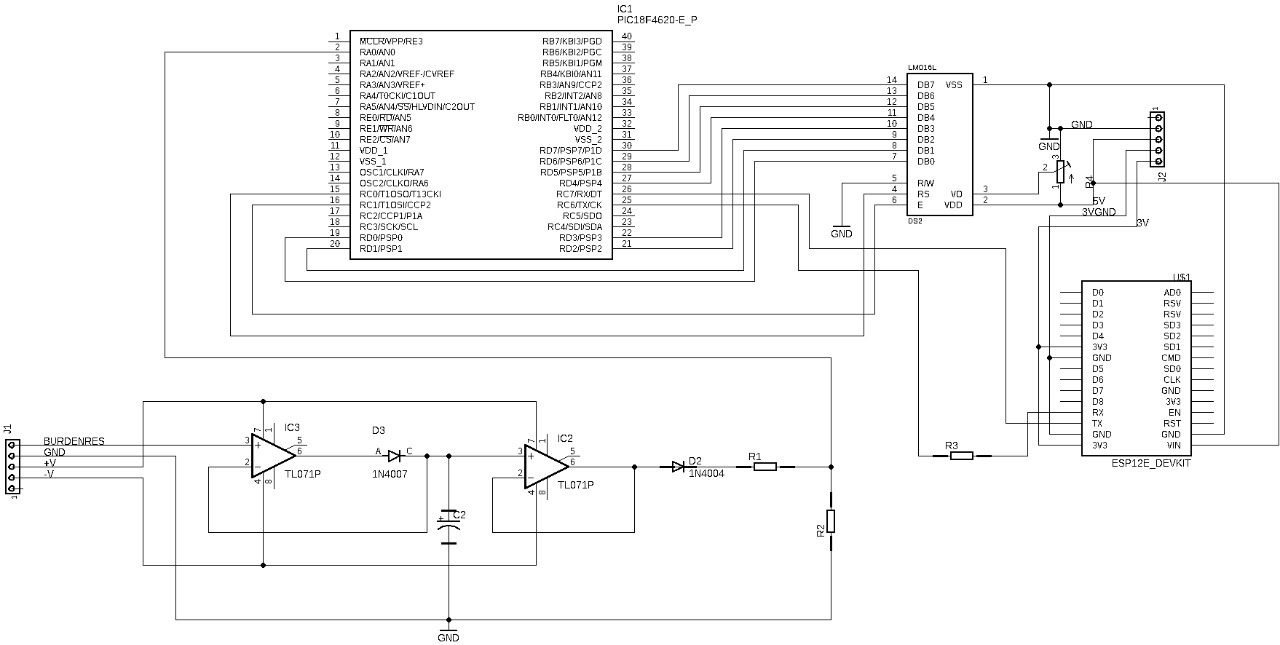
\includegraphics[width=\linewidth]{flow_chart.jpeg}\\
	\caption{System Architecture}
	\label{fig:5.1.1}
\end{figure}
\begin{center}
Figure \ref{fig:5.1.1} Show System Architecture
\end{center}

\subsubsection{Collection of Controllers \& sensors}

\begin{itemize}
	\item Pic Microcontroller 
	\item  CT Sensor 
	\item 1- channel 12 Volt relay module 
	\item LCD 16 x 2 Display
	\item PICKIT 3
	\item NodeMCU 
\end{itemize}

\pagebreak
\subsubsection{Software Design of Project}

\begin{itemize}
	\item Initialize the enter output pin of the pic controller.
	\item Initialize SSID and NodeMCU Password.
	\item Initialization of Firebase Channel Keys.
	\item Initiate the LCD.
	\item Sensor calibration (Sensor value= Sensor value/1.five).
	\item Transmit your information to Firebase.
	\item Serial conversation among the NodeMCU and the controller.
\end{itemize}

\subsubsection{Hardware design of Project}

\begin{itemize}
	\item Interface sensor and LCD  to pic controller.
	\item Set up serial conversation among the NodeMCU and the controller. 
	\item Design of the circuit of the relay driver.
	\item Sensor calibration.
	\item Integrating general hardware.
\end{itemize}

\subsubsection{Hardware and software program integration of Project}

\begin{itemize}
	\item Dump the Pic code to the controller.
	\item Connect Pic with NodeMCU. 
	\item Dump firebase connection code in NodeMCU.
	\item Create your Firebase channel.
	\item Using this write and examine API keys date is despatched to Firebase.
\end{itemize}

\subsubsection{Cloud connectivity and Mobile App improvement}

\begin{itemize}
	\item  Retrieve information from the Firebase app this is saved in a real-time database.
	\item Use the write key and examine key with the right channel ID. 
	\item Create the primary display screen for the utility with the emblem at the flash display screen.
	\item Main pastime with 4 alternatives On / Off, strength reading, notification, etc.
	\item Shows usages in card view.
	\item On/Off pastime- two buttons with excessive and coffee enter API write keys.
	\item Reading pastime-Calculation of strength for each 1 second.
\end{itemize}

\subsection{Project Flowchart}
\textbf{Project glide is given in beneath diagram how diverse pastime are finished and the way statistics is switch amongst them.
}\\

\begin{figure}[H]
	\centering
	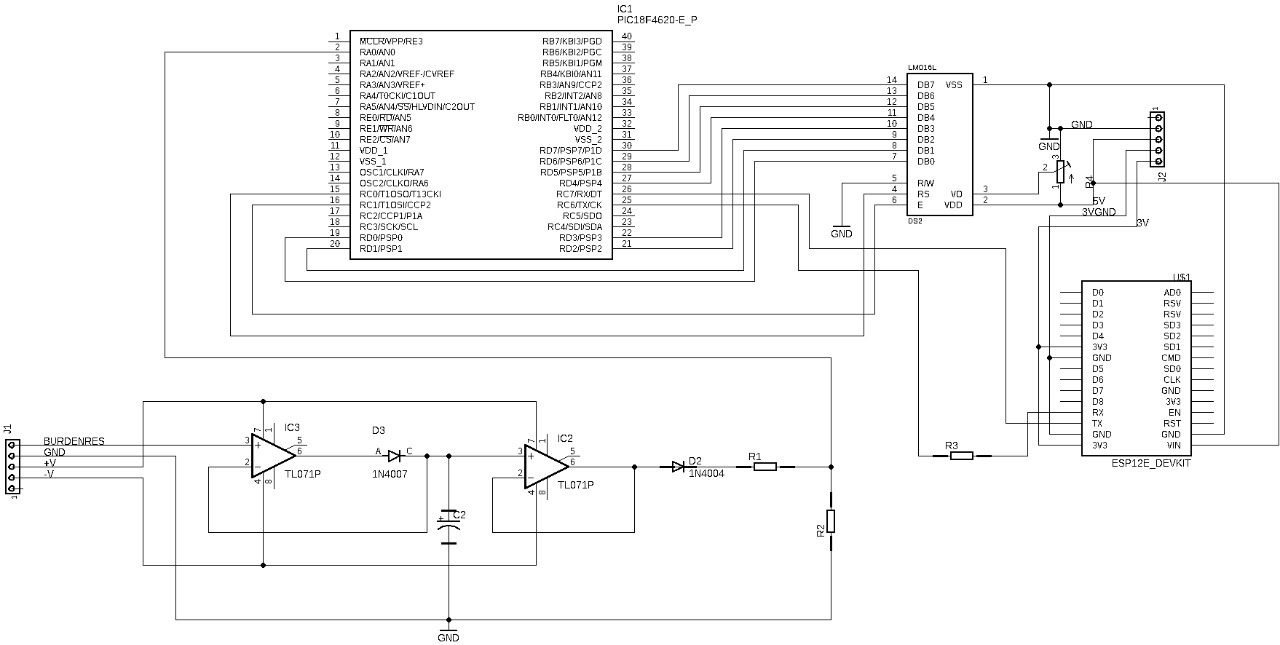
\includegraphics[width=\linewidth]{flow_chart.jpeg}\\
	\caption{Project Flowchart \& Serial communication}
	\label{fig 5.2}
\end{figure}
\begin{center}
Figure \ref{fig 5.2} Show Project Flowchart \& Serial communication
\end{center}

\subsection{Design Specifications of Connections}

\begin{itemize}
	\item Use Firebase, LCD, software program serial libraries for Pic controller.
	\item By Connecting sensors to analog (A1)  enter pin of controller.
	\item Connect NodeMCU module Rx and Tx to Tx and Rx pin of controller.
	\item Connect LCD pins to virtual ouput pins 1 to five and 11, 12.
	\item Digital out pin  thirteen to ULN IC (Relay driver).
	\item Use flash display in android app.
	\item Card view for  interest display.
	\item Use lecho library and graph view. 
	\item Use volley library and Firebase library.
\end{itemize}

\subsection{Serial communication}
\hspace{0.5cm}Connection of pins to PIC controller and the NodeMCU is as proven in table.\\


\textbf{Connections:}\\

\begin{table}[h!]
  \begin{center}
    \begin{tabular}{|c|c|r|p{1.7cm}|}
     \hline
    PIC & NodeMCU\\
    \hline
    VCC & CHPD\\
    \hline
    GND & GND\\
    \hline
    3.3V & VCC\\
    \hline
    VCC & Reset\\
    \hline
    Rx & Tx\\
    \hline
    Tx & Rx\\
    \hline
  \end{tabular}
  \caption{Connections }
  \label{tab:table1}
 \end{center}
\end{table}
\begin{center}
The table \ref{tab:table1} Connections
\end{center}


% -----------------                    Chapter  6. RESULTS AND DISCUSSION             ------------------------------

\newpage
\pagebreak
\vspace*{\fill}% * is needed here
\noindent
\makebox[\textwidth]{\textbf{\huge Chapter  6. RESULTS \& DISCUSSIONS}}
\vfill


\newpage
\section{RESULTS \& DISCUSSIONS OF THE PROJECT}
\fancyfoot[R]{\thepage}

\hspace{0.5cm}Once we activate the mains, the gadget will start. All electric gadget might be on and the contemporary sinter will sense the contemporary in analog form. We can put up it to the picture. Pic has integrated ADC (analog to virtual converter). The quantity of energy is measured and despatched to the firebase the use of NodeMCU. Firebase records is then acquired withinside the android software and visible withinside the cart from those readings. \\


\subsection{Firebase result}
\hspace{0.5cm}We create a channel in the Firebase interface and create two fields. According to the data submitted, the results are displayed in the real-time database. Like users data, calculated power \& controller nodes.\\

\begin{figure}[H]
	\centering
	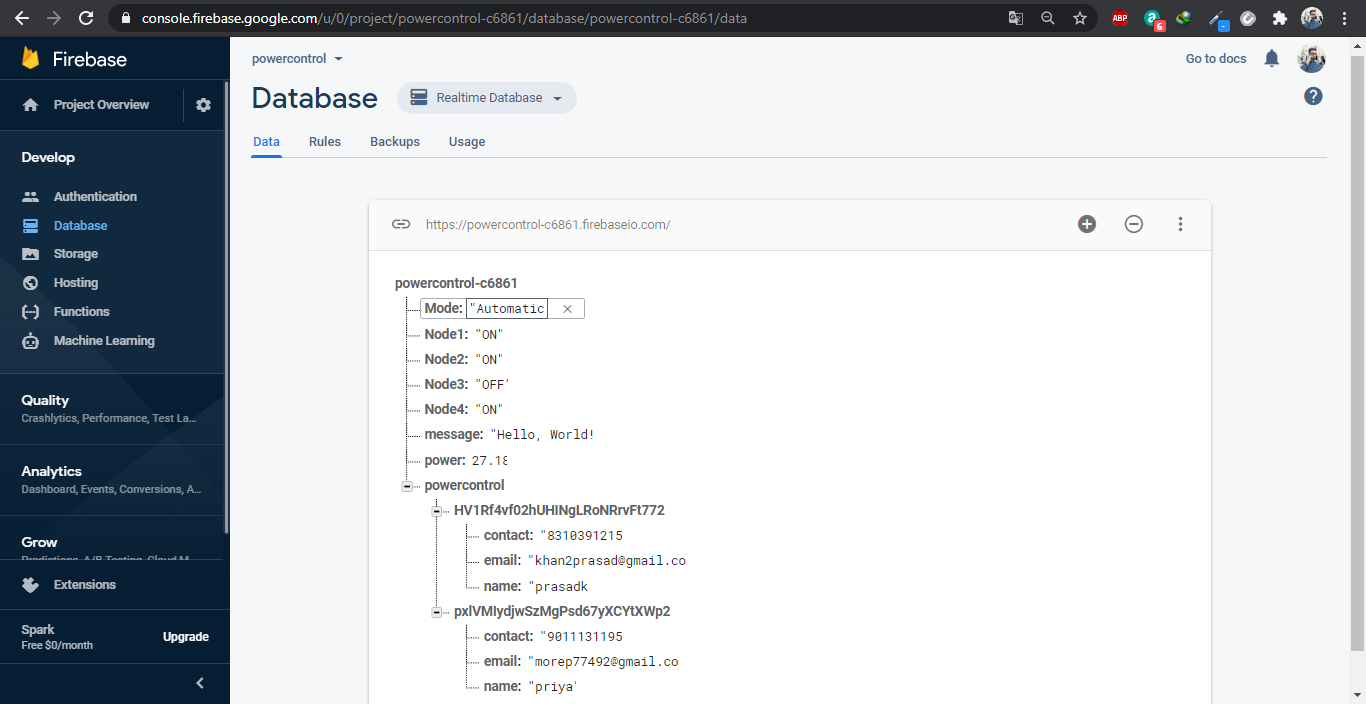
\includegraphics[width=\linewidth]{fbdb1.PNG}\\
	\caption{Firebase results}
	\label{fig:6.1}
\end{figure}
\begin{center}
Figure \ref{fig:6.1} Show Firebase results.
\end{center}

\subsection{Android App result}
\hspace{0.5cm}The Android application fetches the Firebase data as a read and displays it under the read tab of the Android application. We use read api kThe Android software fetches the Firebase records as a study and presentations it below the study tab of the Android software. We use study api key to study the records. The following facts display all of the results of the android applications. And we also can controller the strength utilization through the usage of controller node buttons.ey to read the data. The following statistics show all the outcomes of the android applications. And we can also controller the power usage by using controller node buttons.\\

\begin{figure}[H]
	\centering
	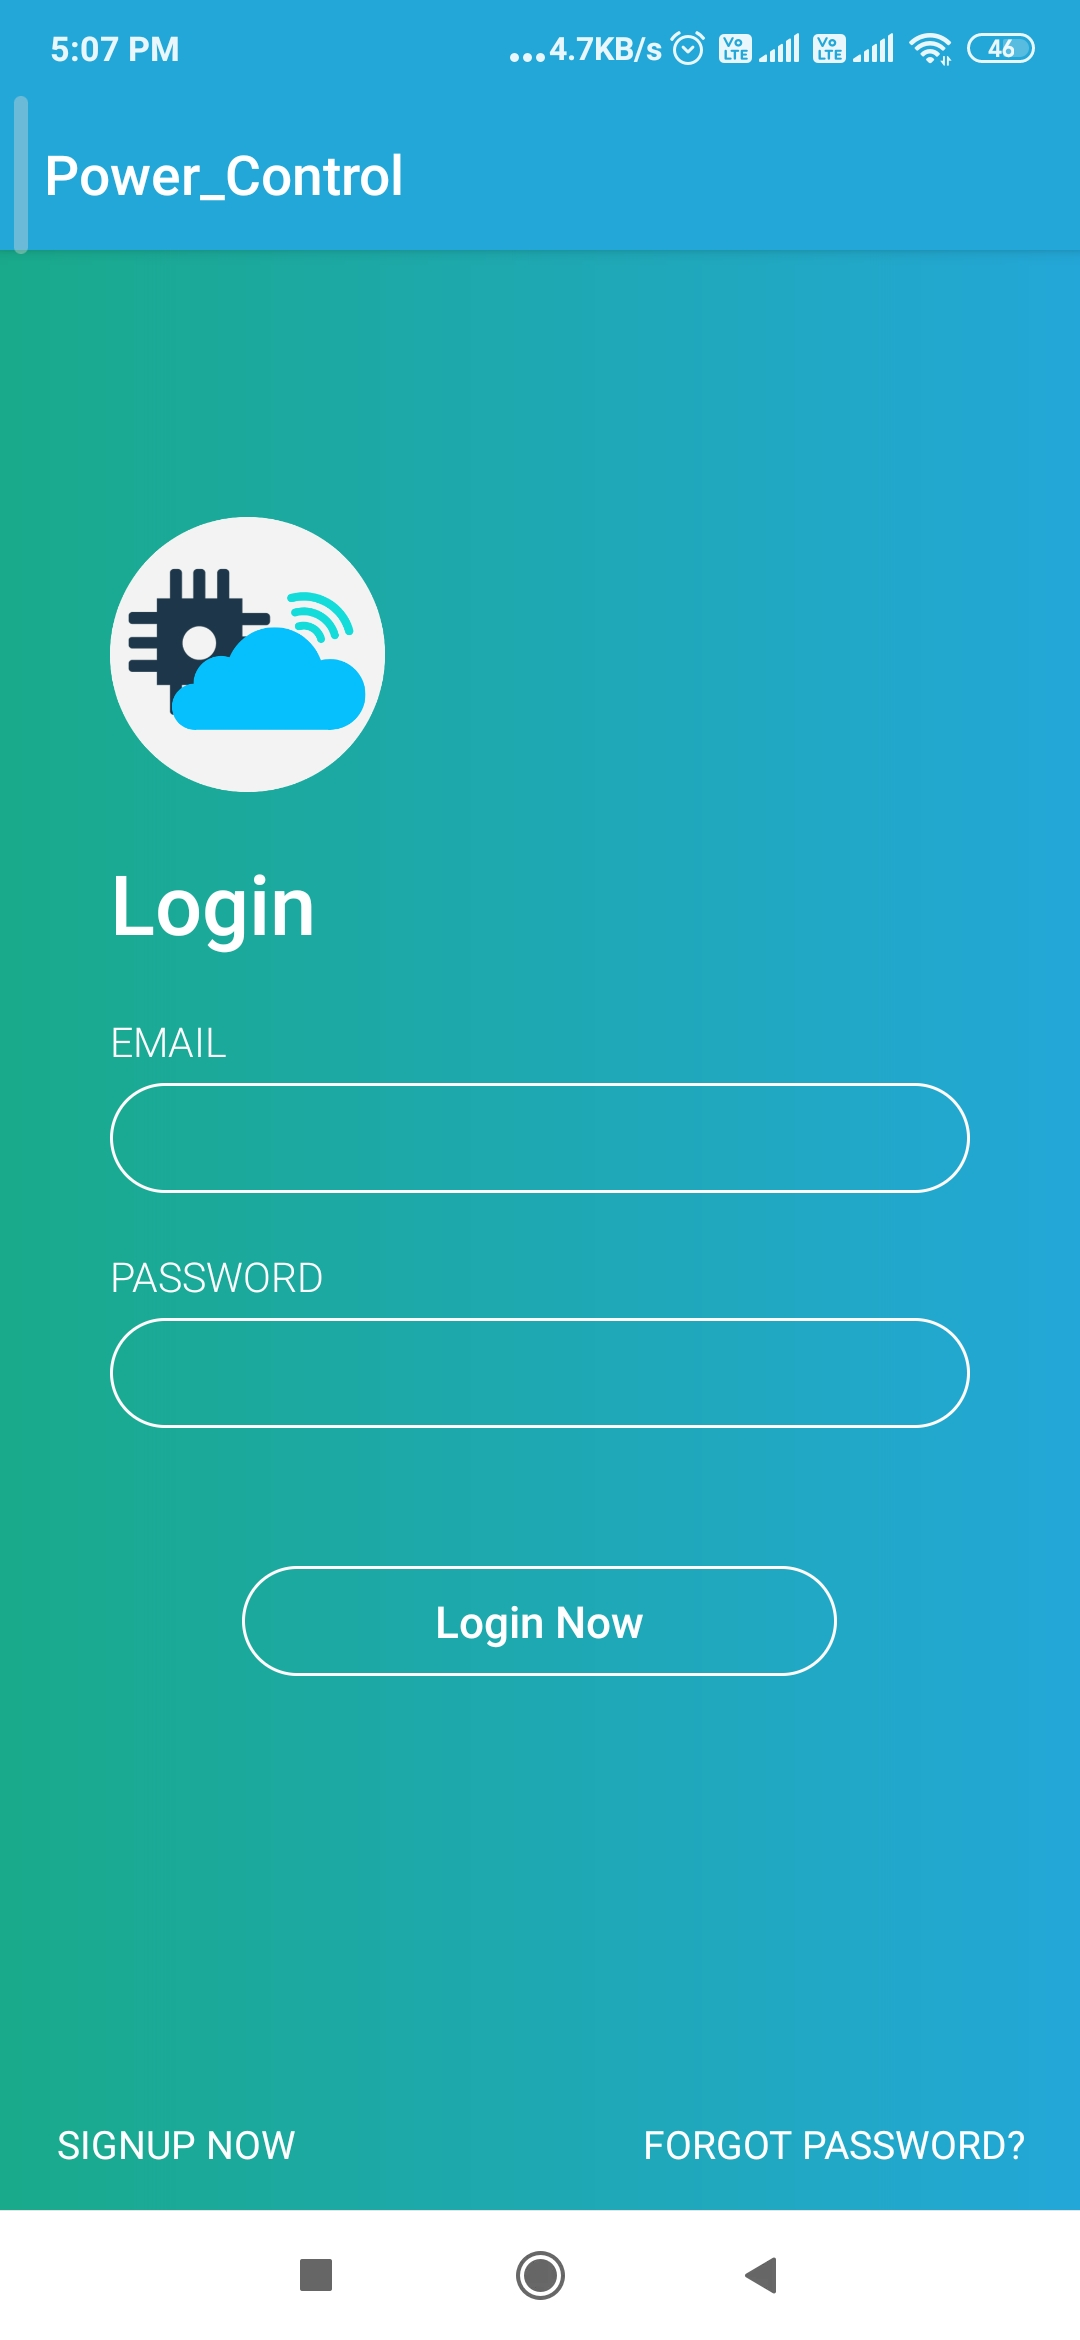
\includegraphics[width=5cm, height=9cm]{appi2.jpg}\\
	\caption{App Log in form }
	\label{fig:6.2.1}
\end{figure}
\begin{center}
Figure \ref{fig:6.2.1} Show Login of App.
\end{center}

\begin{figure}[H]
	\centering
	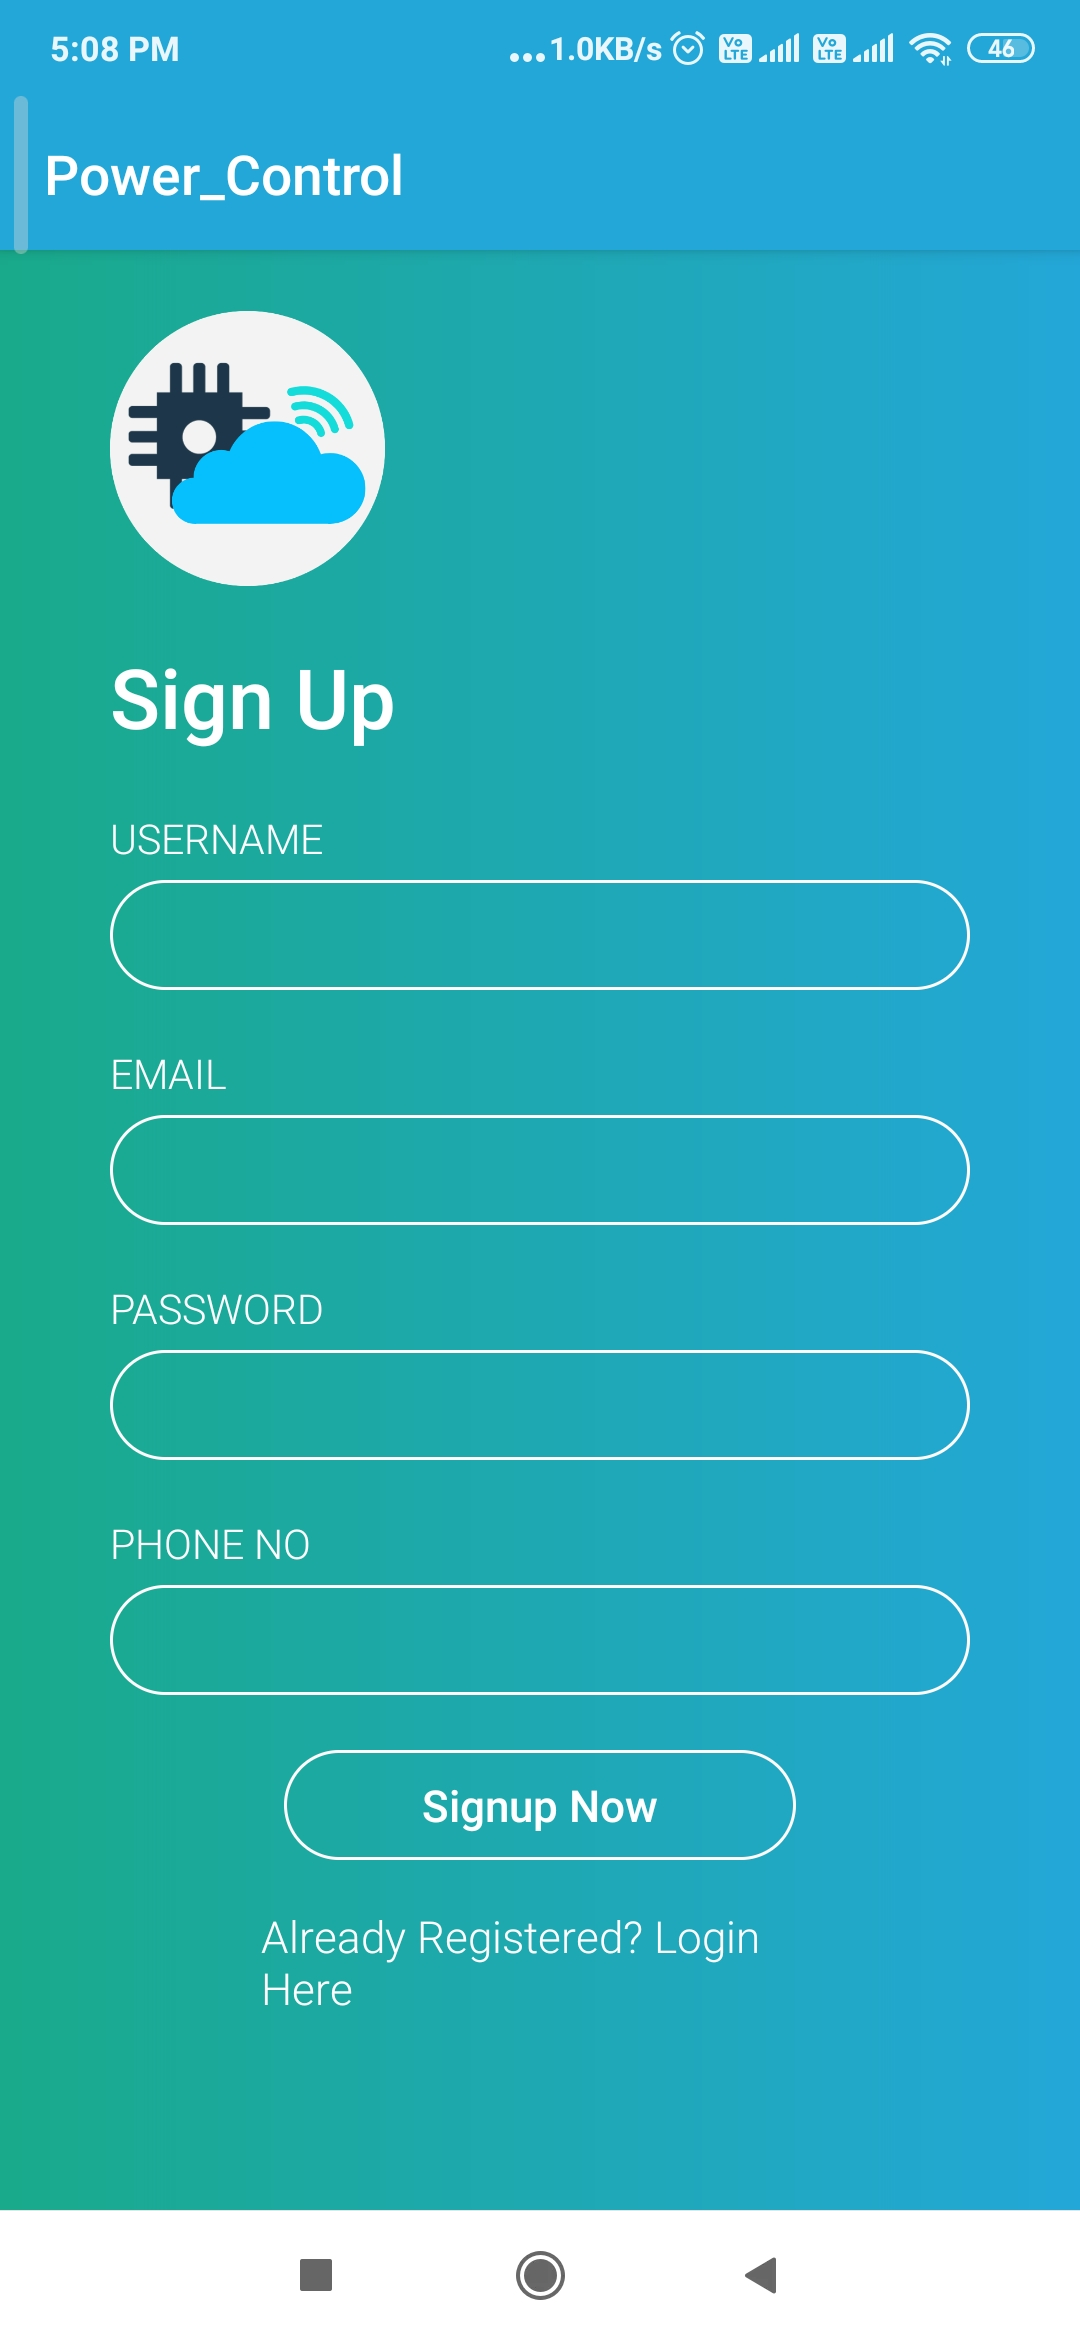
\includegraphics[width=5cm, height=9cm]{appi3.jpg}\\
	\caption{App Registration form}
	\label{fig:6.2.2}
\end{figure}
\begin{center}
Figure \ref{fig:6.2.2} Show Sign Up of App.
\end{center}

\begin{figure}[H]
	\centering
	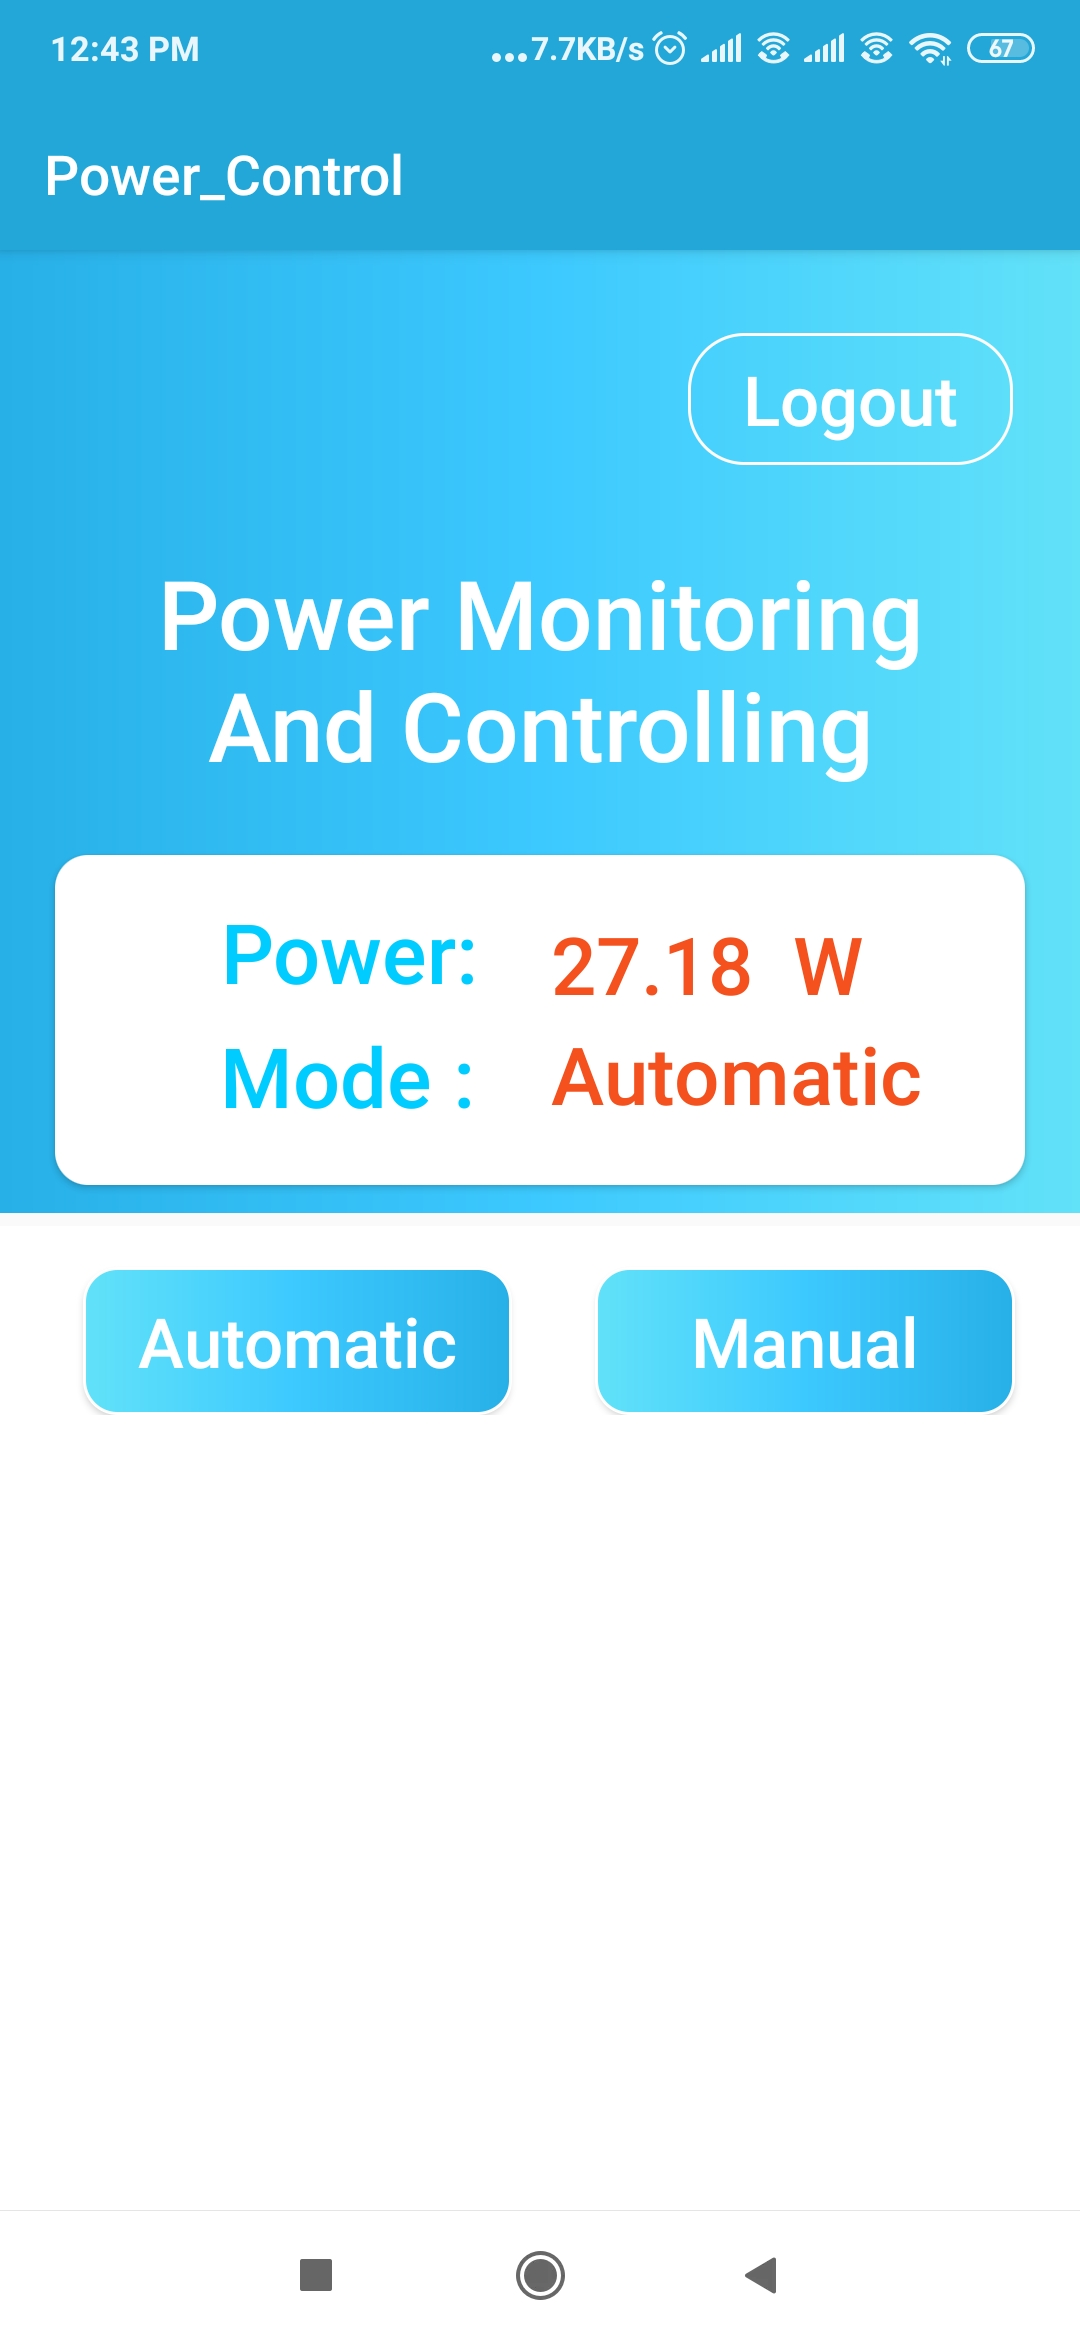
\includegraphics[width=5cm, height=9cm]{appi6.jpg}\\
	\caption{Automatic Mode }
	\label{fig:6.2.3}
\end{figure}
\begin{center}
Figure \ref{fig:6.2.3} Show Automatic Mode.
\end{center}

\begin{figure}[H]
	\centering
	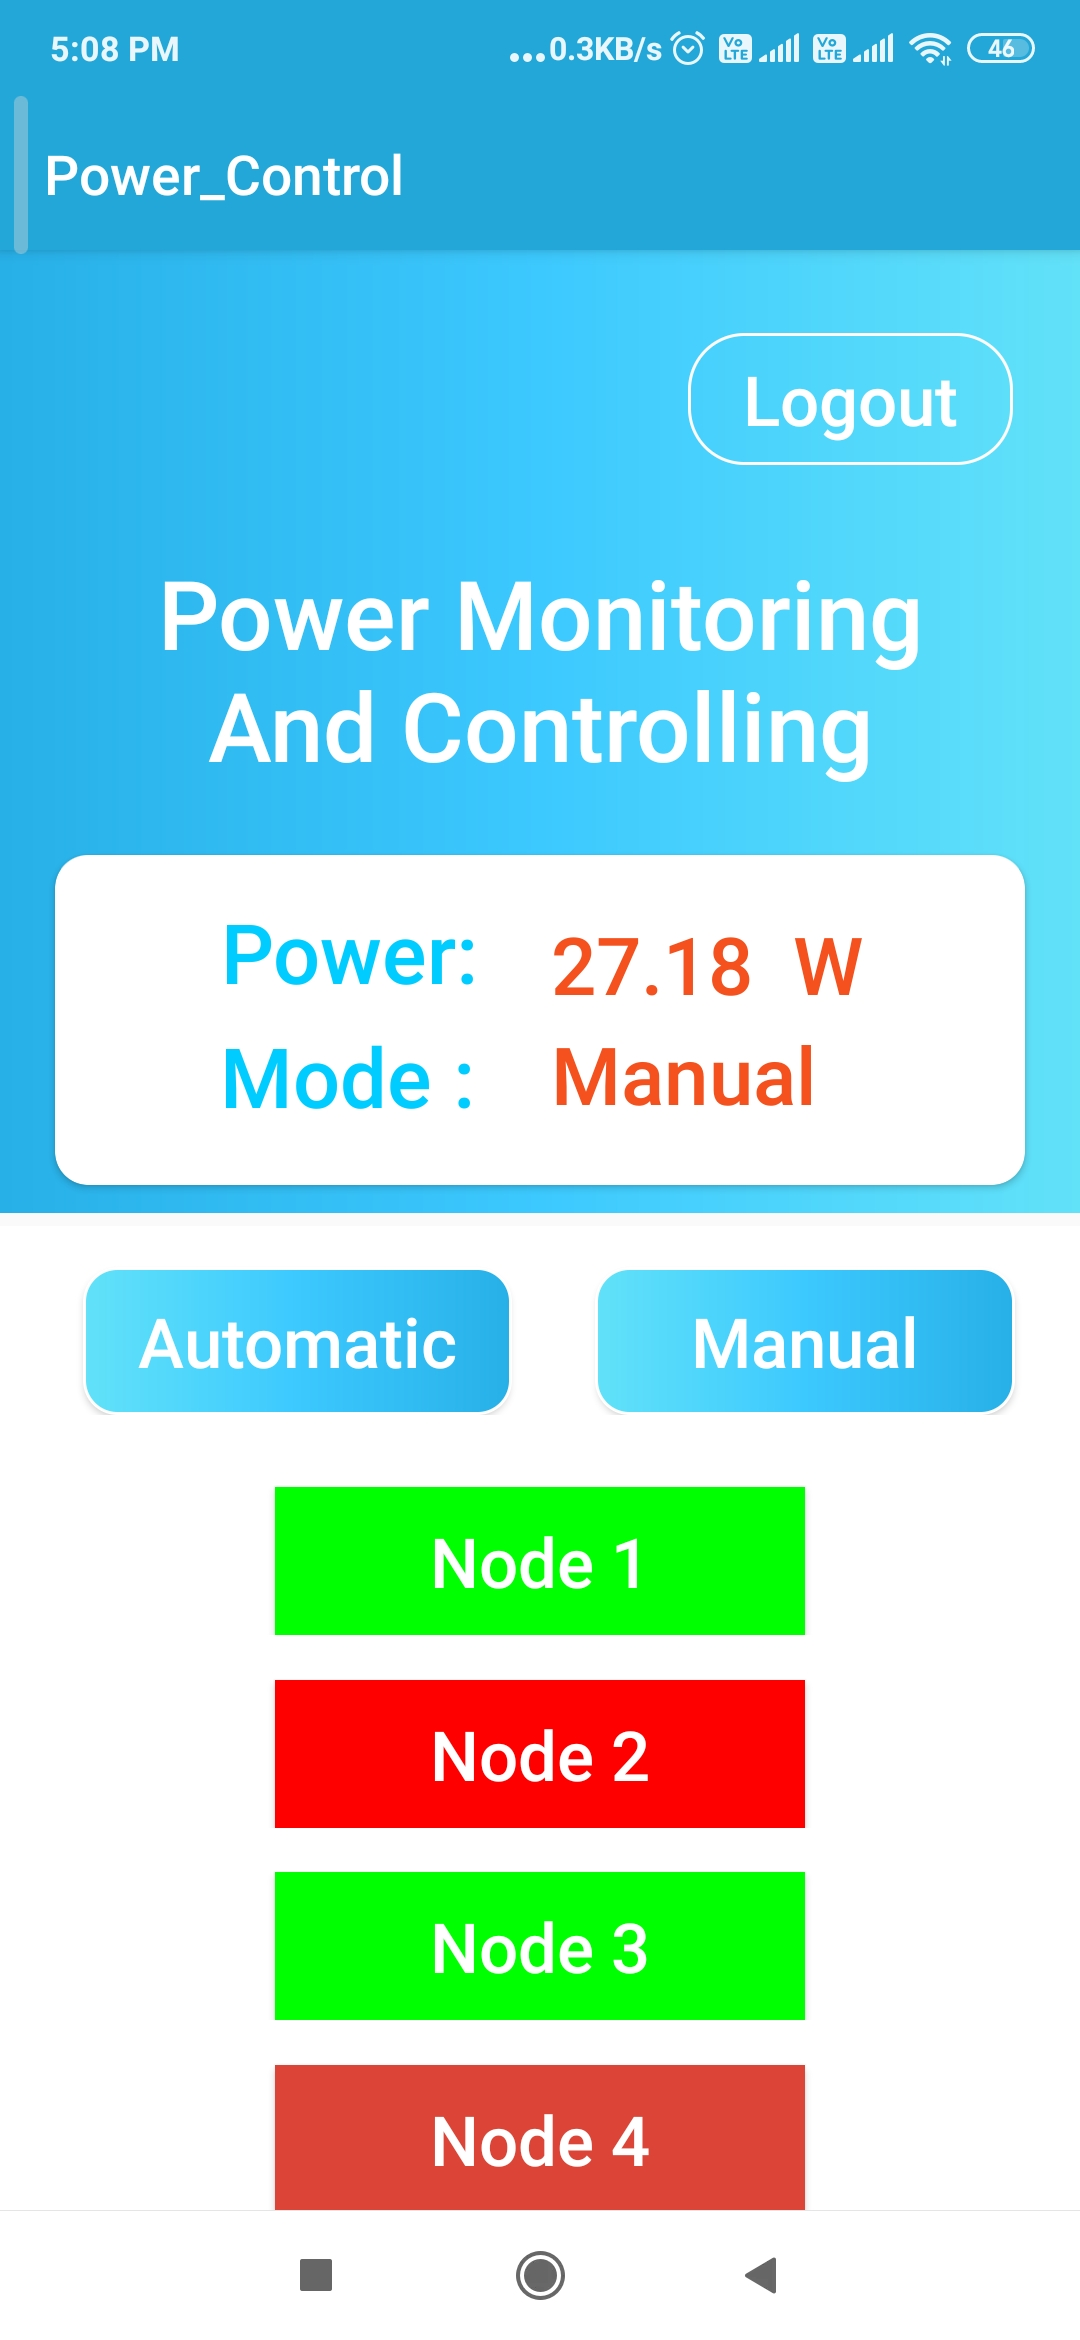
\includegraphics[width=5cm, height=9cm]{appi5.jpg}\\
	\caption{Manual Mode}
	\label{fig:6.2.4}
\end{figure}
\begin{center}
Figure \ref{fig:6.2.4} Show Manual Mode.
\end{center}

\subsection{Analysis of actual reading}
\vspace{0.1in}
\textbf{\large{All above figures suggests suggests the readings for 3 days in conjunction with blunders factor.}}\\

% -----------------                    Chapter  7. Conclusion and future enhancement          ------------------------------

\newpage
\pagebreak
\vspace*{\fill}% * is needed here
\noindent
\makebox[\textwidth]{\textbf{\huge Conclusion \& Future Directions}}
\vfill


\newpage
\section{Conclusion and future Advancements}
\fancyfoot[R]{\thepage}

\hspace{0.5cm}Smart electricity tracking and controlling machine primarily based totally on IoT is a modern software of this virtual era. The evolved machine offer a example energy calculation along side each day energy intake file along side faraway tracking of electrical home equipment and controlling it.\\

For contemporary detecting we right here used Current transformer evaluate to different gadgets it green and we will switch information to firebase cloud the use of NodeMCU.\\

Firebase cloud offer a great UI additionally shops information in xsl and json layout as a result fetching that information in android software end up smooth via way of means of the use of numerous extraordinary library of android studio (IDE for cellular software development).\\

Present machine notify consumer approximately energy utilization and facility of remotely on/off however destiny change make it lots green and reliable.\\


\subsection{Future Directions of the Project}

\begin{itemize}
	\item Efficiency may be elevated the use of uses like gallileo boards and texas board.
	\item Enhance the machine via way of means of including functions like price of invoice from android software.
	\item The graphical data concerning the electricity utilization will be despatched to the consumer in a less difficult layout with the assist of device learning.
	\item Use device and AI and advocate manner of energy intake for a selected area.
	\item The machine will be to be had for industrial reason for massive scale.
\end{itemize}

\subsection{References of the Project}

\hspace{0.5cm} \textbf{7.2.1} We referd papar which is Design and implementation of Bluetooth energy meter (2012)
By P. Shum, H. W. Kuek. for understanding the cenario of electricity usages and consumption. Where they used for digital meter for checking energy usages And all the collected data can be collected by user sending data by using bluetooth wirelessly.\\

\hspace{0.2cm} \textbf{7.2.2} Survey checking from IoT Based Energy Meter Reading, Theft Detection and Disconnection the use of PLC modem and Power optimization”, (Vol. 4, Issue 7, July 2015). The given energy meter machine reduces or almost removes the human involvement in electricity management. It is likewise useful in time period of pay of power invoice due to vital server is there. The consumer can screen and managed power intake in gadgets from an internet interface via way of means of supplying IP deal with of devices. this machine additionally can be used for detection theft of power and tempering with power checking meter.\\

\hspace{0.2cm} \textbf{7.2.3} Birendra Kumar Sahani 1, Tejashree Ravi 2, Aqib Javed Tamboli 3, Ranjeet Pisal four
They posted IRJET on April four 2017.\\

\hspace{0.2cm} \textbf{7.2.4} Gowthami. P Gunasundari. N and Gobinath. S Worked on IOT Based Energy Meter PIC Microcontroller calculating price and displayed in display board and serial communique has been used to interface with the digital terminal.

\end{document}